% =====================================================================
%  Chapter 9: Gradients, Hessians, and Optimization
%  Sections 9.1 and 9.2
% =====================================================================

\chapter{Gradients, Hessians, and Optimization}
\label{ch:9}

Chapter \ref{ch:8} ended with a quiet test for the highest and lowest nearby values.
If a point is free to move in every direction, then an interior maximum or minimum can
only happen when the first-order change disappears:
\[
    df=\mathbf 0.
\]
For a scalar field, that becomes
\[
    \nabla f=\mathbf 0.
\]

Before we use that condition to find peaks, valleys, and saddle points, we need to look
more closely at what the gradient is doing geometrically.  It is not only a calculator for
directional derivatives.  It is the vector that stands perpendicular to level sets.

\section{The gradient and level sets}
\label{sec:9.1}

Recall from Section \ref{sec:7.2} that the gradient gives directional derivatives:
\[
    D_{\mathbf u}f(\mathbf p)=\nabla f(\mathbf p)\cdot \mathbf u.
\]
So if a direction \(\mathbf u\) produces no first-order change in \(f\), then
\[
    \nabla f(\mathbf p)\cdot \mathbf u=0.
\]
That one dot product explains why gradients cross contour lines at right angles.

\subsection{A contour line on a hill}

Picture a hill behind an observatory.  Let \(x\) measure meters east and \(y\) measure
meters north.  Suppose the height is modeled by
\[
    h(x,y)=100+4x+3y-x^2-xy-y^2.
\]
At the point
\[
    P=(1,0),
\]
the height is
\[
    h(1,0)=100+4-1=103.
\]
So \(P\) lies on the contour line
\[
    h(x,y)=103.
\]

The gradient is
\[
    \nabla h(x,y)=\left(4-2x-y,\ 3-x-2y\right).
\]
At \(P=(1,0)\),
\[
    \nabla h(1,0)=(2,2).
\]

Now suppose a hiker starts at \(P\) and walks along the contour line \(h=103\).
Along that walk, the height does not change.  So any tangent direction to the contour
must give directional derivative \(0\).  If
\[
    \mathbf v=(a,b)
\]
is a tangent vector at \(P\), then
\[
    \nabla h(P)\cdot \mathbf v=0.
\]
Here that says
\[
    (2,2)\cdot(a,b)=0,
\]
or
\[
    2a+2b=0.
\]
Thus
\[
    a+b=0.
\]
One tangent direction is
\[
    (1,-1).
\]

The tangent line through \(P=(1,0)\) is therefore
\[
    (x,y)=(1,0)+t(1,-1),
\]
or
\[
\boxed{
    x+y=1.
}
\]

\begin{figure}[h]
\centering
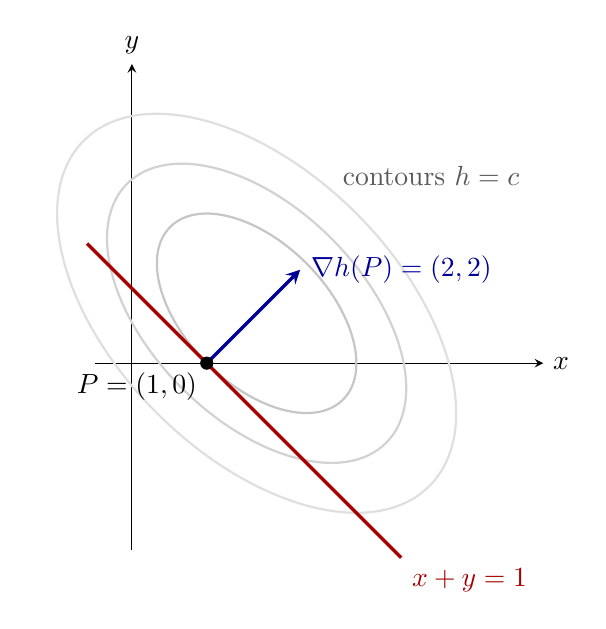
\begin{tikzpicture}[scale=0.95, >=stealth]
    \draw[->] (-0.5,0) -- (5.5,0) node[right] {\(x\)};
    \draw[->] (0,-2.5) -- (0,4.0) node[above] {\(y\)};

    \coordinate (C) at (1.667,0.667);
    \coordinate (P) at (1,0);

    \begin{scope}[rotate around={45:(C)}]
        % Corrected dimensions to precisely intersect P(1,0) and fix the stretch orientation
        \draw[gray!45, thick] (C) ellipse (0.943 and 1.633);
        \draw[gray!35, thick] (C) ellipse (1.414 and 2.449);
        \draw[gray!25, thick] (C) ellipse (1.886 and 3.266);
    \end{scope}

    \draw[very thick, red!65!black] (-0.6,1.6) -- (3.6,-2.6)
        node[below right] {\(x+y=1\)};

    \draw[->, very thick, blue!60!black] (P) -- ++(1.25,1.25)
        node[right] {\(\nabla h(P)=(2,2)\)};

    \fill (P) circle (2.5pt);
    \node[below left] at (P) {\(P=(1,0)\)};

    \node[gray!70!black] at (4.0,2.5) {contours \(h=c\)};
\end{tikzpicture}
\caption{The gradient points normal to the contour line.  The tangent direction gives
zero first-order change.}
\end{figure}

Notice what the tangent line is saying.  It is not saying that the whole straight line
\(x+y=1\) stays on the same contour.  In fact, if we move along that line by writing
\[
    (x,y)=(1+t,-t),
\]
then
\[
    h(1+t,-t)=103-t^2.
\]
The height changes by a second-order amount.  The tangent line only captures the
first-order behavior of the contour at \(P\).

That is exactly what a tangent line should do.

\subsection{The gradient as normal to a level curve}

The example gives the general pattern.

Suppose
\[
    f(x,y)=c
\]
is a level curve, and suppose a differentiable parametrization of part of the curve is
\[
    \mathbf r(t)=(x(t),y(t)).
\]
Since the curve stays on one level set,
\[
    f(\mathbf r(t))=c
\]
for all \(t\).  Differentiate both sides with respect to \(t\).  The left side uses the chain
rule from Section \ref{sec:8.1}:
\[
    \frac{d}{dt}f(\mathbf r(t))
    =
    \nabla f(\mathbf r(t))\cdot \mathbf r'(t).
\]
The right side is constant, so its derivative is \(0\).  Therefore
\[
\boxed{
    \nabla f(\mathbf r(t))\cdot \mathbf r'(t)=0.
}
\]
The velocity vector \(\mathbf r'(t)\) is tangent to the level curve.  The gradient is
orthogonal to it.

\begin{theorem}[Gradient normal to a level curve]
Let \(f\) be differentiable near a point
\[
    \mathbf p=(a,b),
\]
and suppose
\[
    \nabla f(\mathbf p)\ne \mathbf 0.
\]
If the level set
\[
    f(x,y)=f(a,b)
\]
is a smooth curve near \(\mathbf p\), then
\[
\boxed{
    \nabla f(\mathbf p)
}
\]
is normal to the level curve at \(\mathbf p\).

The tangent line is
\[
\boxed{
    \nabla f(\mathbf p)\cdot \bigl((x,y)-\mathbf p\bigr)=0.
}
\]
In coordinates,
\[
\boxed{
    f_x(a,b)(x-a)+f_y(a,b)(y-b)=0.
}
\]
\end{theorem}

\begin{proof}
Let
\[
    \mathbf r(t)
\]
be a differentiable parametrization of the level curve, with
\[
    \mathbf r(t_0)=\mathbf p.
\]
Since
\[
    f(\mathbf r(t))=f(\mathbf p),
\]
the chain rule gives
\[
    \nabla f(\mathbf r(t_0))\cdot \mathbf r'(t_0)=0.
\]
Thus the gradient is perpendicular to the tangent direction.  A line through
\(\mathbf p\) with normal vector \(\nabla f(\mathbf p)\) has equation
\[
    \nabla f(\mathbf p)\cdot \bigl((x,y)-\mathbf p\bigr)=0.
\]
\end{proof}

The condition
\[
    \nabla f(\mathbf p)\ne\mathbf 0
\]
is not decoration.  Without it, the level set may fail to have one clean tangent line.

\begin{example}[Why the nonzero-gradient condition is needed]
Let
\[
    f(x,y)=x^2-y^2.
\]
At the origin,
\[
    \nabla f(0,0)=(0,0).
\]
The level set
\[
    f(x,y)=0
\]
is
\[
    x^2-y^2=0,
\]
so
\[
    (x-y)(x+y)=0.
\]
Thus the level set is the crossing of two lines:
\[
    y=x
    \qquad\text{and}\qquad
    y=-x.
\]

At the origin there is no single tangent line to the whole level set.  One branch has
tangent direction \((1,1)\), and the other has tangent direction \((1,-1)\).

The zero gradient warned us that the ordinary tangent-line picture might break.
\end{example}

A different failure can also happen.  For
\[
    f(x,y)=x^2+y^2,
\]
the level set
\[
    f(x,y)=0
\]
is only the single point \((0,0)\).  Again
\[
    \nabla f(0,0)=\mathbf 0,
\]
and there is no ordinary curve to draw.

When the gradient is nonzero, the implicit function theorem from Chapter \ref{ch:8}
says the level set really does behave locally like a smooth curve.  The tangent formula
then tells us its first-order direction.

\subsection{The gradient as normal to a level surface}

The same reasoning works in space.

Suppose
\[
    F(x,y,z)=c
\]
is a level surface.  A curve
\[
    \mathbf r(t)=(x(t),y(t),z(t))
\]
lying on that surface satisfies
\[
    F(\mathbf r(t))=c.
\]
Differentiating gives
\[
    \nabla F(\mathbf r(t))\cdot \mathbf r'(t)=0.
\]
Every tangent direction to the surface is perpendicular to the gradient.

\begin{example}[A tangent plane to an ellipsoidal shell]
A thin ellipsoidal shell is modeled by the level surface
\[
    F(x,y,z)=x^2+2y^2+3z^2=6.
\]
The point
\[
    P=(1,1,1)
\]
lies on the shell because
\[
    1^2+2(1)^2+3(1)^2=6.
\]

The gradient is
\[
    \nabla F(x,y,z)=(2x,4y,6z),
\]
so
\[
    \nabla F(1,1,1)=(2,4,6).
\]
This is a normal vector to the surface at \(P\).

The tangent plane is
\[
    (2,4,6)\cdot\bigl((x,y,z)-(1,1,1)\bigr)=0.
\]
So
\[
    2(x-1)+4(y-1)+6(z-1)=0.
\]
Dividing by \(2\),
\[
\boxed{
    x+2y+3z=6.
}
\]
\end{example}

\begin{theorem}[Gradient normal to a level surface]
Let \(F\) be differentiable near
\[
    \mathbf p=(a,b,c),
\]
and suppose
\[
    \nabla F(\mathbf p)\ne\mathbf 0.
\]
If the level set
\[
    F(x,y,z)=F(a,b,c)
\]
is a smooth surface near \(\mathbf p\), then
\[
\boxed{
    \nabla F(\mathbf p)
}
\]
is normal to the surface at \(\mathbf p\).

The tangent plane is
\[
\boxed{
    \nabla F(\mathbf p)\cdot \bigl((x,y,z)-\mathbf p\bigr)=0.
}
\]
In coordinates,
\[
\boxed{
    F_x(a,b,c)(x-a)+F_y(a,b,c)(y-b)+F_z(a,b,c)(z-c)=0.
}
\]
\end{theorem}

In the language of differentials, the same statement is shorter.  A tangent vector
\[
    \mathbf v
\]
to the level surface must satisfy
\[
\boxed{
    dF_{\mathbf p}(\mathbf v)=0.
}
\]
Since
\[
    dF=F_x\,dx+F_y\,dy+F_z\,dz,
\]
this says
\[
    F_x(a,b,c)v_1+F_y(a,b,c)v_2+F_z(a,b,c)v_3=0.
\]
The tangent plane is the set of first-order motions that \(dF\) sends to zero.

\subsection{Orthogonality of flow lines and contours}

Contour maps show level curves.  The gradient points across them.

If a hiker walks in the direction of steepest uphill motion, the velocity is parallel to
\[
    \nabla h.
\]
If rainwater runs downhill, its velocity is often modeled as parallel to
\[
    -\nabla h.
\]
Either way, the motion crosses contours at right angles, because each contour's tangent
direction is perpendicular to the gradient.

A curve satisfying
\[
    \mathbf r'(t)=\nabla f(\mathbf r(t))
\]
is called a \emph{gradient flow line}.  Along such a curve,
\[
\begin{aligned}
    \frac{d}{dt}f(\mathbf r(t))
    &=
    \nabla f(\mathbf r(t))\cdot \mathbf r'(t)\\
    &=
    \nabla f(\mathbf r(t))\cdot \nabla f(\mathbf r(t))\\
    &=
    \|\nabla f(\mathbf r(t))\|^2.
\end{aligned}
\]
So unless the gradient is zero, \(f\) increases along its own gradient flow.

For downhill flow,
\[
    \mathbf r'(t)=-\nabla f(\mathbf r(t)),
\]
we get
\[
    \frac{d}{dt}f(\mathbf r(t))
    =
    -\|\nabla f(\mathbf r(t))\|^2.
\]
So \(f\) decreases unless the gradient is zero.

This is a beautiful place for the story to pause.  Level curves show where the function
is constant.  Gradient flow lines show the directions where the function changes as fast
as possible.  But both descriptions lose their direction when
\[
    \nabla f=\mathbf 0.
\]
At such a point, first-order motion goes silent.  The point might be the top of a hill,
the bottom of a bowl, or a mountain pass.  Those silent points are where optimization
begins.

\section{Critical points}
\label{sec:9.2}

Section \ref{sec:9.1} ended at the places where the gradient disappears.  A gradient
flow line has no direction there.  A contour map may pinch, cross, or close up there.
For optimization, those points are the first ones we must find.

\subsection{A hill with a highest nearby point}

Return to the hill
\[
    h(x,y)=100+4x+3y-x^2-xy-y^2.
\]
Its gradient is
\[
    \nabla h(x,y)=\left(4-2x-y,\ 3-x-2y\right).
\]
Set the gradient equal to zero:
\[
    4-2x-y=0,
    \qquad
    3-x-2y=0.
\]
Equivalently,
\[
    2x+y=4,
    \qquad
    x+2y=3.
\]
Solving gives
\[
    y=\frac23,
    \qquad
    x=\frac53.
\]
So first-order change disappears at
\[
    P=\left(\frac53,\frac23\right).
\]

At that point,
\[
    h(P)=\frac{313}{3}.
\]
To see what kind of point it is, write
\[
    x=\frac53+u,
    \qquad
    y=\frac23+v.
\]
A direct substitution gives
\[
\boxed{
    h\left(\frac53+u,\frac23+v\right)
    =
    \frac{313}{3}-(u^2+uv+v^2).
}
\]
Now
\[
    u^2+uv+v^2
    =
    \left(u+\frac12v\right)^2+\frac34v^2.
\]
This is always nonnegative, and it is zero only when
\[
    u=0,\qquad v=0.
\]
Therefore every nearby point has height at most
\[
    \frac{313}{3},
\]
with equality only at \(P\).  The point \(P\) is a local maximum.

The gradient equation found the candidate.  The completed square told us what kind of
candidate it was.

\subsection{Local maxima and minima}

The word \emph{local} means nearby.  A local maximum does not have to be the highest
point in the whole domain.  It only has to be the highest point in some small region
around the point.

\begin{definition}[Local maximum and local minimum]
Let
\[
    f:D\subseteq\mathbb R^n\to\mathbb R.
\]
A point \(\mathbf p\in D\) is a \emph{local maximum} of \(f\) if there is some radius
\(r>0\) such that
\[
    f(\mathbf x)\le f(\mathbf p)
\]
for every \(\mathbf x\in D\) with
\[
    \|\mathbf x-\mathbf p\|<r.
\]

A point \(\mathbf p\in D\) is a \emph{local minimum} of \(f\) if there is some radius
\(r>0\) such that
\[
    f(\mathbf x)\ge f(\mathbf p)
\]
for every \(\mathbf x\in D\) with
\[
    \|\mathbf x-\mathbf p\|<r.
\]

A local maximum or local minimum is called a \emph{local extremum}.
\end{definition}

\begin{example}[A quiet spot in a sound model]
Suppose the loudness near a quiet spot in a room is modeled by
\[
    L(x,y)=5+(x-2)^2+3(y+1)^2.
\]
At
\[
    (2,-1),
\]
we have
\[
    L(2,-1)=5.
\]
Every other nearby point gives
\[
    (x-2)^2+3(y+1)^2>0.
\]
So
\[
    L(x,y)>5
\]
nearby, except at \((2,-1)\) itself.  Thus \((2,-1)\) is a local minimum.

The gradient agrees:
\[
    \nabla L(x,y)=\left(2(x-2),6(y+1)\right),
\]
so
\[
    \nabla L(2,-1)=\mathbf 0.
\]
\end{example}

\subsection{Saddle points}

A critical point does not have to be a maximum or a minimum.

Consider the mountain-pass model
\[
    S(x,y)=80+x^2-y^2.
\]
The gradient is
\[
    \nabla S(x,y)=(2x,-2y).
\]
At the origin,
\[
    \nabla S(0,0)=\mathbf 0.
\]
But the origin is not a local maximum or a local minimum.

Along the \(x\)-axis,
\[
    S(x,0)=80+x^2,
\]
which is larger than \(80\) when \(x\ne0\).  Along the \(y\)-axis,
\[
    S(0,y)=80-y^2,
\]
which is smaller than \(80\) when \(y\ne0\).

So every small disk around the origin contains points higher than the origin and points
lower than the origin.  This is a saddle point.

\begin{figure}[h]
\centering
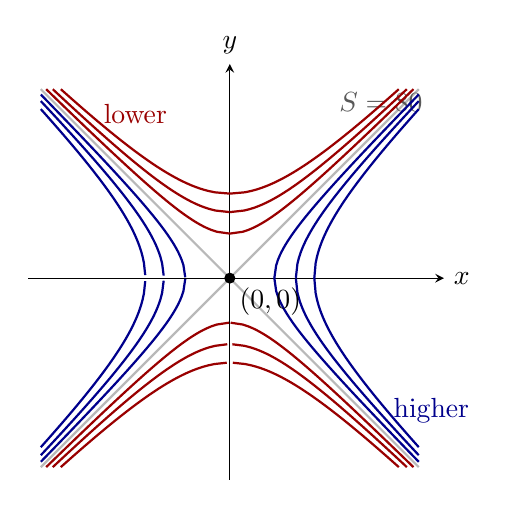
\begin{tikzpicture}[scale=0.8, >=stealth]
    \draw[->] (-3.2,0) -- (3.4,0) node[right] {\(x\)};
    \draw[->] (0,-3.2) -- (0,3.4) node[above] {\(y\)};

    \draw[thick, gray!55] (-3,-3) -- (3,3);
    \draw[thick, gray!55] (-3,3) -- (3,-3);
    \node[gray!70!black] at (2.4,2.8) {\(S=80\)};

   \foreach \c in {0.5,1.1,1.8} {
    \draw[blue!55!black, thick, domain={sqrt(\c)}:3, samples=80]
        plot (\x,{sqrt(abs(\x*\x-\c))});
    \draw[blue!55!black, thick, domain={sqrt(\c)}:3, samples=80]
        plot (\x,{-sqrt(abs(\x*\x-\c))});
    \draw[blue!55!black, thick, domain=-3:{-sqrt(\c)}, samples=80]
        plot (\x,{sqrt(abs(\x*\x-\c))});
    \draw[blue!55!black, thick, domain=-3:{-sqrt(\c)}, samples=80]
        plot (\x,{-sqrt(abs(\x*\x-\c))});

    \draw[red!60!black, thick, domain={sqrt(\c)}:3, samples=80]
        plot ({sqrt(abs(\x*\x-\c))}, \x);
    \draw[red!60!black, thick, domain={sqrt(\c)}:3, samples=80]
        plot ({-sqrt(abs(\x*\x-\c))}, \x);
    \draw[red!60!black, thick, domain=-3:{-sqrt(\c)}, samples=80]
        plot ({sqrt(abs(\x*\x-\c))}, \x);
    \draw[red!60!black, thick, domain=-3:{-sqrt(\c)}, samples=80]
        plot ({-sqrt(abs(\x*\x-\c))}, \x);
}

    \fill (0,0) circle (2.5pt);
    \node[below right] at (0,0) {\((0,0)\)};

    \node[blue!55!black] at (3.2,-2.1) {higher};
    \node[red!60!black] at (-1.5,2.6) {lower};
\end{tikzpicture}
\caption{Near a saddle point, some directions go up and others go down.}
\end{figure}

\begin{definition}[Saddle point]
A point \(\mathbf p\) is a \emph{saddle point} of \(f\) if \(\mathbf p\) is a critical
point and every small ball around \(\mathbf p\) contains points where \(f\) is larger
than \(f(\mathbf p)\) and points where \(f\) is smaller than \(f(\mathbf p)\).
\end{definition}

The saddle point is the first warning that
\[
    \nabla f=\mathbf 0
\]
does not mean ``maximum'' or ``minimum.''  It means that the first-order test has gone
silent.  We need more information to classify the point.

\subsection{Critical points from \texorpdfstring{\(\nabla f=0\)}{grad f = 0}}

Single-variable calculus had Fermat's theorem: if a differentiable function has a local
maximum or minimum at an interior point, then its derivative is zero.  The same idea
works in several variables by looking at one coordinate slice at a time.

\begin{theorem}[Fermat's theorem for functions of several variables]
Let
\[
    f:D\subseteq\mathbb R^n\to\mathbb R.
\]
Suppose \(\mathbf p\) is an interior point of \(D\), and suppose \(f\) has a local
maximum or local minimum at \(\mathbf p\).

If all first partial derivatives of \(f\) exist at \(\mathbf p\), then
\[
\boxed{
    \nabla f(\mathbf p)=\mathbf 0.
}
\]
Equivalently,
\[
\boxed{
    df_{\mathbf p}=0.
}
\]
\end{theorem}

\begin{proof}
Write
\[
    \mathbf p=(p_1,\ldots,p_n).
\]
Hold every variable fixed except \(x_i\).  This gives a one-variable slice through
\(\mathbf p\):
\[
    g_i(t)=f(p_1,\ldots,p_{i-1},t,p_{i+1},\ldots,p_n).
\]
Since \(f\) has a local maximum or minimum at \(\mathbf p\), the slice \(g_i\) has a
local maximum or minimum at
\[
    t=p_i.
\]
By the one-variable Fermat theorem,
\[
    g_i'(p_i)=0.
\]
But
\[
    g_i'(p_i)=f_{x_i}(\mathbf p).
\]
So every first partial derivative is zero.
\end{proof}

This theorem gives necessary conditions, not sufficient ones.  Local maxima and minima
must occur among the points where the first-order test fails, but not every such point is
an extremum.

\begin{definition}[Critical point]
Let
\[
    f:D\subseteq\mathbb R^n\to\mathbb R.
\]
An interior point \(\mathbf p\in D\) is called a \emph{critical point} of \(f\) if either

\[
    \nabla f(\mathbf p)=\mathbf 0,
\]
or one of the first partial derivatives fails to exist at \(\mathbf p\).

When \(f\) is differentiable, the critical points are exactly the interior points where
\[
    \nabla f=\mathbf 0.
\]
\end{definition}

The definition includes points where derivatives fail to exist because extrema can hide
there.

\begin{example}[A sharp peak]
The function
\[
    f(x,y)=-|x|-|y|
\]
has a local maximum at the origin.  But
\[
    f_x(0,0)
\]
does not exist, since along the \(x\)-axis
\[
    f(h,0)=-|h|.
\]
The one-variable derivative of \(-|h|\) at \(0\) does not exist.

So the origin must still be checked in an optimization problem, even though
\[
    \nabla f(0,0)
\]
does not exist.
\end{example}

The hypotheses in Fermat's theorem cannot be dropped.

\begin{example}[Why the point must be interior]
Let
\[
    f(x,y)=x
\]
on the closed disk
\[
    D=\{(x,y):x^2+y^2\le1\}.
\]
The maximum value occurs at
\[
    (1,0),
\]
because no point in the disk has \(x>1\).  But
\[
    \nabla f(1,0)=(1,0),
\]
not \(\mathbf 0\).

There is no contradiction.  The point \((1,0)\) is a boundary point, not an interior
point.  At the boundary, many directions are not allowed.  The function would increase
if we moved farther east, but the disk does not allow that move.
\end{example}

\begin{example}[Why the partial derivatives must exist]
The function
\[
    f(x,y)=-|x|-|y|
\]
has a local maximum at the origin, but the first partial derivatives do not exist there.
So Fermat's theorem does not apply.

The theorem says: if the derivatives exist at an interior local extremum, then they must
be zero.  If the derivatives do not exist, the point is still a candidate.
\end{example}

\subsection{Finding and reading critical points}

Here is a small example where the critical equation finds more than one point.

Let
\[
    f(x,y)=x^3-3x+y^2.
\]
Then
\[
    f_x(x,y)=3x^2-3,
    \qquad
    f_y(x,y)=2y.
\]
Set both equal to zero:
\[
    3x^2-3=0,
    \qquad
    2y=0.
\]
Thus
\[
    x=\pm1,
    \qquad
    y=0.
\]
The critical points are
\[
    (1,0)
    \qquad\text{and}\qquad
    (-1,0).
\]

At \((1,0)\), write
\[
    x=1+u,\qquad y=v.
\]
Then
\[
\begin{aligned}
f(1+u,v)
&=(1+u)^3-3(1+u)+v^2\\
&=-2+3u^2+u^3+v^2\\
&=-2+u^2(3+u)+v^2.
\end{aligned}
\]
For \(|u|<1\),
\[
    3+u>0.
\]
So nearby,
\[
    f(1+u,v)\ge -2,
\]
with equality only at \(u=v=0\).  Thus \((1,0)\) is a local minimum.

At \((-1,0)\), write
\[
    x=-1+u,\qquad y=v.
\]
Then
\[
\begin{aligned}
f(-1+u,v)
&=(-1+u)^3-3(-1+u)+v^2\\
&=2-3u^2+u^3+v^2.
\end{aligned}
\]
Along the line \(u=0\),
\[
    f(-1,v)=2+v^2,
\]
which is larger than \(2\) for \(v\ne0\).  Along the line \(v=0\),
\[
    f(-1+u,0)=2-3u^2+u^3.
\]
For small nonzero \(u\), this is less than \(2\).  So \((-1,0)\) is a saddle point.

This classification was possible by hand, but it took separate local algebra around each
point.  The next sections will build a faster tool for this job.

\subsection{Boundary points must be checked separately}

Critical points are interior candidates.  Boundary points have their own rules, because
not every direction is available.

A rectangular roof is described by
\[
    0\le x\le 4,
    \qquad
    0\le y\le 3.
\]
Suppose sunlight intensity on the roof is modeled by
\[
    B(x,y)=3x+2y.
\]
The gradient is
\[
    \nabla B=(3,2),
\]
so there are no interior critical points.

But the function still has a maximum and a minimum on the rectangle.  Since
\[
    B(x,y)
\]
increases as \(x\) increases and also as \(y\) increases, the minimum occurs at
\[
    (0,0),
\]
and the maximum occurs at
\[
    (4,3).
\]
The values are
\[
    B(0,0)=0,
    \qquad
    B(4,3)=18.
\]

The maximum is not detected by
\[
    \nabla B=\mathbf 0
\]
because the maximum occurs at a corner.  The direction of increasing sunlight points
northeast, but at the corner \((4,3)\) the roof ends.

So an optimization problem on a region has two kinds of candidates:

\[
\begin{array}{c|c}
\text{interior candidates} & \nabla f=\mathbf 0 \text{ or derivatives fail}\\[1mm]
\text{boundary candidates} & \text{optimize on the boundary separately}
\end{array}
\]

For a rectangular boundary, this usually means checking four edges and four corners.
For a circular boundary, it means optimizing along a circle.  For a surface constraint,
it means something subtler: the gradient of \(f\) may not be zero, but it must be
perpendicular to every motion allowed by the constraint.

We have found the first-order candidates.  What we do not yet have is a reliable way to
tell peak from valley from saddle without inventing a new trick each time.  The missing
information is hidden in the second-order part of the local approximation.  In one
variable, that information was \(f''\).  In two variables, it becomes a matrix of second
partials: the Hessian.
\section{Second derivatives and the Hessian matrix}
\label{sec:9.3}

Section \ref{sec:9.2} ended at critical points.  At those points,
\[
    df=\mathbf 0,
\]
so the first-order approximation stops talking.  If a point is a peak, a valley, or a
saddle, that information must come from the next visible part of the function.

That next part is second order.

\subsection{The summit we already met}

Return to the hill from Sections \ref{sec:9.1} and \ref{sec:9.2}:
\[
    h(x,y)=100+4x+3y-x^2-xy-y^2.
\]
Its critical point is
\[
    P=\left(\frac53,\frac23\right).
\]
In Section \ref{sec:9.2}, we wrote
\[
    x=\frac53+u,
    \qquad
    y=\frac23+v,
\]
and found the exact formula
\[
    h\left(\frac53+u,\frac23+v\right)
    =
    \frac{313}{3}-(u^2+uv+v^2).
\]
There is no linear part.  The first visible change is
\[
    -(u^2+uv+v^2).
\]

That expression tells the shape.  Since
\[
    u^2+uv+v^2
    =
    \left(u+\frac12v\right)^2+\frac34v^2,
\]
it is positive unless
\[
    u=v=0.
\]
So every nonzero nearby displacement lowers the height.  The critical point is a local
maximum.

Now look at the second derivatives:
\[
    h_x=4-2x-y,
    \qquad
    h_y=3-x-2y.
\]
Differentiating again gives
\[
    h_{xx}=-2,
    \qquad
    h_{xy}=-1,
    \qquad
    h_{yx}=-1,
    \qquad
    h_{yy}=-2.
\]
These four numbers arrange themselves into the matrix
\[
    H_h=
    \begin{pmatrix}
        -2 & -1\\
        -1 & -2
    \end{pmatrix}.
\]
Then
\[
\frac12
\begin{pmatrix}u&v\end{pmatrix}
\begin{pmatrix}
        -2 & -1\\
        -1 & -2
\end{pmatrix}
\begin{pmatrix}u\\v\end{pmatrix}
=
-(u^2+uv+v^2).
\]
So the second-order part of the hill is stored in a matrix.

That matrix is called the Hessian.

\subsection{Second partial derivatives}

A first partial derivative measures a coordinate slope.  A second partial derivative
measures how that coordinate slope changes.

For a function
\[
    f(x,y),
\]
we have four second partial derivatives:
\[
    f_{xx},
    \qquad
    f_{xy},
    \qquad
    f_{yx},
    \qquad
    f_{yy}.
\]
The notation means
\[
    f_{xy}
    =
    \frac{\partial}{\partial y}\left(f_x\right).
\]
So \(f_{xy}\) means: first differentiate with respect to \(x\), then differentiate the
result with respect to \(y\).

\begin{definition}[Second partial derivatives]
Let
\[
    f:D\subseteq\mathbb R^2\to\mathbb R.
\]
The second partial derivatives of \(f\) are
\[
    f_{xx}=(f_x)_x,
    \qquad
    f_{xy}=(f_x)_y,
    \qquad
    f_{yx}=(f_y)_x,
    \qquad
    f_{yy}=(f_y)_y,
\]
when these derivatives exist.
\end{definition}

\begin{example}[Changing marginal costs]
Recall the bakery cost model
\[
    C(u,v)=400+3u+4v+0.01uv,
\]
where \(u\) is the number of sourdough loaves and \(v\) is the number of rye loaves.

The first partial derivatives are
\[
    C_u=3+0.01v,
    \qquad
    C_v=4+0.01u.
\]
Now differentiate again:
\[
    C_{uu}=0,
    \qquad
    C_{uv}=0.01,
\]
and
\[
    C_{vu}=0.01,
    \qquad
    C_{vv}=0.
\]

The number
\[
    C_{uv}=0.01
\]
says that if the bakery makes one more rye loaf, then the marginal cost of making
sourdough rises by \(0.01\) dollars.  The interaction term \(0.01uv\) is responsible.
Without it, the two products would not affect each other's marginal costs.
\end{example}

\begin{example}[Second partials in three variables]
Let
\[
    T(x,y,z)=18+\frac{4}{1+x^2+y^2}-0.7z.
\]
Then
\[
    T_z=-0.7,
\]
so
\[
    T_{zz}=0.
\]
The temperature changes linearly with height, so the height-slope does not change as
height changes.

For the \(x\)-direction,
\[
    T_x=-\frac{8x}{(1+x^2+y^2)^2}.
\]
A second derivative such as
\[
    T_{xy}
\]
measures how this \(x\)-slope changes as we move in the \(y\)-direction.
\end{example}

Second partial derivatives are rates of change of rates of change.  They are the
multivariable version of \(f''\).

\subsection{Mixed partials and why order usually does not matter}

Two of the second partials are mixed:
\[
    f_{xy}
    \qquad\text{and}\qquad
    f_{yx}.
\]
At first, they look like different operations.  One changes \(x\) first and \(y\) second.
The other changes \(y\) first and \(x\) second.

For ordinary smooth formulas, they are equal.

\begin{example}[Two orders, one answer]
Let
\[
    f(x,y)=x^2y+3xy^2.
\]
Then
\[
    f_x=2xy+3y^2,
\]
so
\[
    f_{xy}=2x+6y.
\]
Also,
\[
    f_y=x^2+6xy,
\]
so
\[
    f_{yx}=2x+6y.
\]
Thus
\[
    f_{xy}=f_{yx}.
\]
\end{example}

This equality is not a coincidence.  It is a theorem, but the theorem needs a regularity
condition.

\begin{theorem}[Equality of mixed partials]
Let \(f\) be defined near a point
\[
    (a,b).
\]
Suppose the mixed partial derivatives
\[
    f_{xy}
    \qquad\text{and}\qquad
    f_{yx}
\]
exist near \((a,b)\) and are continuous at \((a,b)\).  Then
\[
\boxed{
    f_{xy}(a,b)=f_{yx}(a,b).
}
\]
\end{theorem}

\begin{proof}[Proof idea]
Look at the small rectangle with corners
\[
    (a,b),\quad (a+u,b),\quad (a,b+v),\quad (a+u,b+v).
\]
The quantity
\[
\begin{aligned}
    \Delta
    &=
    f(a+u,b+v)-f(a+u,b)\\
    &\qquad
    -f(a,b+v)+f(a,b)
\end{aligned}
\]
measures how much the change in one direction depends on moving in the other
direction.

If we divide by the small signed area \(uv\),
\[
    \frac{\Delta}{uv},
\]
we get an average mixed rate of change over the rectangle.  The one-variable mean
value theorem can read this average in two ways: as an average of \(f_{xy}\), or as an
average of \(f_{yx}\).  As the rectangle shrinks to \((a,b)\), continuity forces both
averages to approach the values at \((a,b)\).  Therefore the two values are equal.
\end{proof}

The continuity assumption is not decoration.  Without it, the two mixed partials can
exist and still disagree.

\begin{example}[Mixed partials can fail to agree]
Define
\[
    F(x,y)=
    \begin{cases}
    \dfrac{xy(x^2-y^2)}{x^2+y^2}, & (x,y)\ne(0,0),\\[3mm]
    0, & (x,y)=(0,0).
    \end{cases}
\]
We will compute the two mixed partials at the origin.

First fix \(y\) and compute \(F_x(0,y)\).  For \(y\ne0\),
\[
\begin{aligned}
F_x(0,y)
&=
\lim_{h\to0}
\frac{F(h,y)-F(0,y)}{h} \\[1mm]
&=
\lim_{h\to0}
\frac{hy(h^2-y^2)}{h(h^2+y^2)}\\[1mm]
&=
\lim_{h\to0}
\frac{y(h^2-y^2)}{h^2+y^2}\\[1mm]
&=
-y.
\end{aligned}
\]
This formula also gives \(F_x(0,0)=0\).  Therefore
\[
    F_x(0,y)=-y.
\]
Now differentiate with respect to \(y\) at \(0\):
\[
    F_{xy}(0,0)
    =
    \lim_{k\to0}\frac{F_x(0,k)-F_x(0,0)}{k}
    =
    \lim_{k\to0}\frac{-k}{k}
    =
    -1.
\]

Now reverse the order.  For \(x\ne0\),
\[
\begin{aligned}
F_y(x,0)
&=
\lim_{k\to0}
\frac{F(x,k)-F(x,0)}{k}\\[1mm]
&=
\lim_{k\to0}
\frac{xk(x^2-k^2)}{k(x^2+k^2)}\\[1mm]
&=
\lim_{k\to0}
\frac{x(x^2-k^2)}{x^2+k^2}\\[1mm]
&=
x.
\end{aligned}
\]
This formula also gives \(F_y(0,0)=0\).  Therefore
\[
    F_y(x,0)=x.
\]
Now differentiate with respect to \(x\) at \(0\):
\[
    F_{yx}(0,0)
    =
    \lim_{h\to0}\frac{F_y(h,0)-F_y(0,0)}{h}
    =
    \lim_{h\to0}\frac{h}{h}
    =
    1.
\]

So
\[
\boxed{
    F_{xy}(0,0)=-1,
    \qquad
    F_{yx}(0,0)=1.
}
\]
The mixed partials exist, but they are not equal.  The missing condition is continuity
of the mixed partials near the origin.
\end{example}

In differential-form language, when \(f\) is smooth enough,
\[
    df=f_x\,dx+f_y\,dy.
\]
Taking \(d\) again gives
\[
    d(df)=(f_{yx}-f_{xy})\,dx\wedge dy.
\]
The equality of mixed partials says
\[
    d(df)=0.
\]
This small cancellation will return later as the rule
\[
    d^2=0.
\]
For now, it tells us why the Hessian of a smooth function is symmetric.

\subsection{The Hessian matrix}

At a point \((a,b)\), collect the second partials into one matrix:
\[
    H_f(a,b)
    =
    \begin{pmatrix}
        f_{xx}(a,b) & f_{xy}(a,b)\\
        f_{yx}(a,b) & f_{yy}(a,b)
    \end{pmatrix}.
\]

\begin{definition}[Hessian matrix in two variables]
For a twice differentiable function
\[
    f(x,y),
\]
the \emph{Hessian matrix} of \(f\) at \((a,b)\) is
\[
\boxed{
    H_f(a,b)
    =
    \begin{pmatrix}
        f_{xx}(a,b) & f_{xy}(a,b)\\
        f_{yx}(a,b) & f_{yy}(a,b)
    \end{pmatrix}.
}
\]
If the second partials are continuous near \((a,b)\), then
\[
    f_{xy}(a,b)=f_{yx}(a,b),
\]
so the Hessian is symmetric.
\end{definition}

For a function of three variables,
\[
    f(x,y,z),
\]
the Hessian is
\[
\boxed{
H_f(a,b,c)
=
\begin{pmatrix}
f_{xx} & f_{xy} & f_{xz}\\
f_{yx} & f_{yy} & f_{yz}\\
f_{zx} & f_{zy} & f_{zz}
\end{pmatrix}_{(a,b,c)}.
}
\]
When the second partials are continuous, this matrix is symmetric across its diagonal.

\begin{example}[The Hessian of the hill]
For
\[
    h(x,y)=100+4x+3y-x^2-xy-y^2,
\]
we found
\[
    h_{xx}=-2,
    \qquad
    h_{xy}=-1,
    \qquad
    h_{yx}=-1,
    \qquad
    h_{yy}=-2.
\]
So
\[
    H_h=
    \begin{pmatrix}
        -2 & -1\\
        -1 & -2
    \end{pmatrix}.
\]
This Hessian is constant because \(h\) is already a quadratic function.
\end{example}

\begin{example}[A Hessian that changes from point to point]
Let
\[
    f(x,y)=x^3-3x+y^2.
\]
Then
\[
    f_x=3x^2-3,
    \qquad
    f_y=2y.
\]
So
\[
    f_{xx}=6x,
    \qquad
    f_{xy}=0,
    \qquad
    f_{yx}=0,
    \qquad
    f_{yy}=2.
\]
The Hessian is
\[
    H_f(x,y)
    =
    \begin{pmatrix}
        6x & 0\\
        0 & 2
    \end{pmatrix}.
\]
At the critical point \((1,0)\),
\[
    H_f(1,0)
    =
    \begin{pmatrix}
        6 & 0\\
        0 & 2
    \end{pmatrix}.
\]
At the critical point \((-1,0)\),
\[
    H_f(-1,0)
    =
    \begin{pmatrix}
        -6 & 0\\
        0 & 2
    \end{pmatrix}.
\]
The same function bends differently at its two critical points.
\end{example}

The Hessian is the matrix version of the second derivative.  To see this, we need the
second-order approximation.

\subsection{Quadratic approximation near a critical point}

In one-variable calculus, Taylor's formula said that near \(a\),
\[
    f(a+h)
    =
    f(a)+f'(a)h+\frac12f''(a)h^2+\text{smaller terms}.
\]
In two variables, the same story has more directions.  Near \((a,b)\), write
\[
    x=a+u,
    \qquad
    y=b+v.
\]
Then the second-order approximation is
\[
\begin{aligned}
f(a+u,b+v)
&\approx
f(a,b)
+
f_x(a,b)u
+
f_y(a,b)v\\
&\qquad
+
\frac12
\left(
f_{xx}(a,b)u^2
+
2f_{xy}(a,b)uv
+
f_{yy}(a,b)v^2
\right).
\end{aligned}
\]

The first line is the linear approximation.  The second line is the quadratic correction.

In matrix form,
\[
\boxed{
f(a+u,b+v)
\approx
f(a,b)
+
df_{(a,b)}(u,v)
+
\frac12
\begin{pmatrix}u&v\end{pmatrix}
H_f(a,b)
\begin{pmatrix}u\\v\end{pmatrix}.
}
\]
At a critical point,
\[
    df_{(a,b)}=0.
\]
So the approximation becomes
\[
\boxed{
f(a+u,b+v)
\approx
f(a,b)
+
\frac12
\begin{pmatrix}u&v\end{pmatrix}
H_f(a,b)
\begin{pmatrix}u\\v\end{pmatrix}.
}
\]

\begin{example}[A minimum seen through its quadratic part]
Let
\[
    f(x,y)=x^3-3x+y^2.
\]
At the critical point
\[
    (1,0),
\]
write
\[
    x=1+u,
    \qquad
    y=v.
\]
Then
\[
\begin{aligned}
f(1+u,v)
&=
(1+u)^3-3(1+u)+v^2\\
&=
-2+3u^2+u^3+v^2.
\end{aligned}
\]
The quadratic part is
\[
    3u^2+v^2.
\]
The Hessian at \((1,0)\) is
\[
    H_f(1,0)
    =
    \begin{pmatrix}
        6&0\\
        0&2
    \end{pmatrix},
\]
and
\[
\frac12
\begin{pmatrix}u&v\end{pmatrix}
\begin{pmatrix}
        6&0\\
        0&2
\end{pmatrix}
\begin{pmatrix}u\\v\end{pmatrix}
=
3u^2+v^2.
\]
So the Hessian gives exactly the quadratic part of the local expansion.
\end{example}

\begin{theorem}[Second-order approximation]
Suppose \(f(x,y)\) has continuous second partial derivatives near \((a,b)\).  Then
\[
\begin{aligned}
f(a+u,b+v)
&=
f(a,b)
+
f_x(a,b)u
+
f_y(a,b)v\\
&\qquad
+
\frac12
\left(
f_{xx}(a,b)u^2
+
2f_{xy}(a,b)uv
+
f_{yy}(a,b)v^2
\right)
+
R(u,v),
\end{aligned}
\]
where the remainder \(R(u,v)\) is small compared with \(u^2+v^2\):
\[
\boxed{
    \frac{R(u,v)}{u^2+v^2}\to0
    \quad\text{as}\quad
    (u,v)\to(0,0).
}
\]
Equivalently,
\[
\boxed{
f((a,b)+\mathbf u)
=
f(a,b)
+
df_{(a,b)}(\mathbf u)
+
\frac12\mathbf u^T H_f(a,b)\mathbf u
+
R(\mathbf u),
}
\]
with
\[
    \frac{R(\mathbf u)}{\|\mathbf u\|^2}\to0.
\]
\end{theorem}

\begin{proof}[Proof idea]
Move from \((a,b)\) to \((a+u,b+v)\) along the straight path
\[
    \mathbf r(t)=(a,b)+t(u,v),
    \qquad 0\le t\le1.
\]
The composite
\[
    g(t)=f(\mathbf r(t))
\]
is a one-variable function.  Taylor's formula for \(g\) at \(t=0\) gives
\[
    g(1)=g(0)+g'(0)+\frac12g''(0)+\text{smaller terms}.
\]
The chain rule gives
\[
    g'(0)=df_{(a,b)}(u,v),
\]
and a second use of the chain rule gives
\[
    g''(0)
    =
    \begin{pmatrix}u&v\end{pmatrix}
    H_f(a,b)
    \begin{pmatrix}u\\v\end{pmatrix}.
\]
This gives the formula.  Continuity of the second partials is what makes the remaining
terms smaller than \(\|\mathbf u\|^2\).
\end{proof}

At a critical point, the first-order part vanishes.  The Hessian becomes the first
visible shape.  But a matrix is not yet an answer.  We still need to know how to read
\[
    \mathbf u^T H\mathbf u.
\]
Can it be positive in every nonzero direction?  Negative in every direction?  Positive
in one direction and negative in another?  Those three possibilities are the mechanism
behind the second derivative test.

\section{The second derivative test}
\label{sec:9.4}

Section \ref{sec:9.3} showed what replaces \(f''\) in several variables.  Near a critical
point,
\[
    f(\mathbf p+\mathbf u)-f(\mathbf p)
\]
is controlled first by
\[
    \frac12\mathbf u^T H_f(\mathbf p)\mathbf u.
\]
So the question becomes a question about a quadratic expression.

\[
    \text{What signs can } \mathbf u^T H\mathbf u \text{ have?}
\]

\subsection{Reading the quadratic part}

Consider the function
\[
    B(x,y)=12+2x^2+xy+y^2.
\]
At the origin,
\[
    B_x=4x+y,
    \qquad
    B_y=x+2y,
\]
so
\[
    \nabla B(0,0)=\mathbf 0.
\]
The origin is a critical point.

The change from the origin is
\[
    B(x,y)-B(0,0)=2x^2+xy+y^2.
\]
Complete the square:
\[
    2x^2+xy+y^2
    =
    2\left(x+\frac14y\right)^2+\frac78y^2.
\]
This is positive unless
\[
    x=y=0.
\]
So
\[
    B(x,y)>B(0,0)
\]
for every nearby nonzero point.  The origin is a local minimum.

Now consider
\[
    M(x,y)=12-2x^2-xy-y^2.
\]
Again the origin is a critical point, but
\[
    M(x,y)-M(0,0)=-(2x^2+xy+y^2).
\]
So every nearby nonzero point gives a smaller value.  The origin is a local maximum.

Finally consider
\[
    S(x,y)=12+x^2-y^2.
\]
At the origin,
\[
    \nabla S(0,0)=\mathbf 0.
\]
But
\[
    S(x,0)=12+x^2>12
\]
for \(x\ne0\), while
\[
    S(0,y)=12-y^2<12
\]
for \(y\ne0\).  The origin is a saddle point.

The three quadratic parts behave differently:
\[
\begin{array}{c|c|c}
\text{Quadratic part} & \text{Sign behavior} & \text{Shape}\\ \hline
2x^2+xy+y^2 & \text{positive for every nonzero direction} & \text{minimum}\\[1mm]
-(2x^2+xy+y^2) & \text{negative for every nonzero direction} & \text{maximum}\\[1mm]
x^2-y^2 & \text{positive in some directions, negative in others} & \text{saddle}
\end{array}
\]

\begin{definition}[Definite and indefinite quadratic forms]
Let \(H\) be a symmetric matrix, and define
\[
    q(\mathbf u)=\mathbf u^T H\mathbf u.
\]

The quadratic form \(q\) is called \emph{positive definite} if
\[
    q(\mathbf u)>0
\]
for every nonzero vector \(\mathbf u\).

It is called \emph{negative definite} if
\[
    q(\mathbf u)<0
\]
for every nonzero vector \(\mathbf u\).

It is called \emph{indefinite} if it takes both positive and negative values.
\end{definition}

The Hessian tells the local shape through its quadratic form.

\begin{figure}[h]
\centering
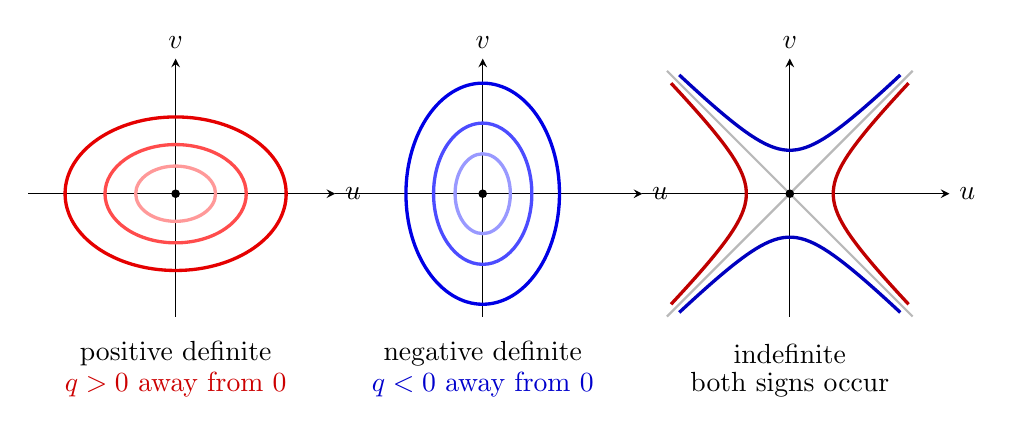
\begin{tikzpicture}[scale=0.78, >=stealth]
    % positive definite panel
    \begin{scope}[xshift=-5.0cm]
        \draw[->] (-2.4,0) -- (2.6,0) node[right] {\(u\)};
        \draw[->] (0,-2.0) -- (0,2.2) node[above] {\(v\)};
        
        % Increasingly saturated red as q gets larger
        \draw[very thick, red!40] (0,0) ellipse (0.65 and 0.45);
        \draw[very thick, red!70] (0,0) ellipse (1.15 and 0.8);
        \draw[very thick, red!90!black] (0,0) ellipse (1.8 and 1.25);
        
        \fill (0,0) circle (2pt);
        \node at (0,-2.6) {positive definite};
        \node[red!80!black] at (0,-3.1) {\(q>0\) away from \(0\)};
    \end{scope}

    % negative definite panel 
    \begin{scope}
        \draw[->] (-2.4,0) -- (2.6,0) node[right] {\(u\)};
        \draw[->] (0,-2.0) -- (0,2.2) node[above] {\(v\)};
        
        % Increasingly saturated blue as q gets more negative
        \draw[very thick, blue!40] (0,0) ellipse (0.45 and 0.65);
        \draw[very thick, blue!70] (0,0) ellipse (0.8 and 1.15);
        \draw[very thick, blue!90!black] (0,0) ellipse (1.25 and 1.8);
        
        \fill (0,0) circle (2pt);
        \node at (0,-2.6) {negative definite};
        \node[blue!80!black] at (0,-3.1) {\(q<0\) away from \(0\)};
    \end{scope}

    % indefinite panel 
    \begin{scope}[xshift=5.0cm]
        \draw[->] (-2.4,0) -- (2.6,0) node[right] {\(u\)};
        \draw[->] (0,-2.0) -- (0,2.2) node[above] {\(v\)};
        \draw[gray!55, thick] (-2,-2) -- (2,2);
        \draw[gray!55, thick] (-2,2) -- (2,-2);

        % Right and Left branches (positive -> red)
        \draw[very thick, red!75!black, domain=-1.8:1.8, samples=50, variable=\y]
            plot ({sqrt(\y*\y+0.5)}, \y);
        \draw[very thick, red!75!black, domain=-1.8:1.8, samples=50, variable=\y]
            plot ({-sqrt(\y*\y+0.5)}, \y);

        % Top and Bottom branches (negative -> blue)
        \draw[very thick, blue!75!black, domain=-1.8:1.8, samples=50, variable=\x]
            plot (\x, {sqrt(\x*\x+0.5)});
        \draw[very thick, blue!75!black, domain=-1.8:1.8, samples=50, variable=\x]
            plot (\x, {-sqrt(\x*\x+0.5)});

        \fill (0,0) circle (2pt);
        \node at (0,-2.6) {indefinite};
        \node at (0,-3.1) {both signs occur};
    \end{scope}
\end{tikzpicture}
\caption{A definite quadratic form has one sign in every nonzero direction.  An
indefinite form has both signs.}
\end{figure}

\subsection{The two-variable determinant shortcut}

For a two-variable function, the Hessian at a point has the form
\[
    H=
    \begin{pmatrix}
        A & B\\
        B & C
    \end{pmatrix}.
\]
Its quadratic form is
\[
    q(u,v)
    =
    \begin{pmatrix}u&v\end{pmatrix}
    \begin{pmatrix}
        A & B\\
        B & C
    \end{pmatrix}
    \begin{pmatrix}u\\v\end{pmatrix}
    =
    Au^2+2Buv+Cv^2.
\]
The number
\[
\boxed{
    \Delta=AC-B^2
}
\]
decides most cases.

If \(A\ne0\), complete the square:
\[
\begin{aligned}
    q(u,v)
    &=
    Au^2+2Buv+Cv^2\\
    &=
    A\left(u+\frac{B}{A}v\right)^2
    +
    \left(C-\frac{B^2}{A}\right)v^2\\
    &=
    A\left(u+\frac{B}{A}v\right)^2
    +
    \frac{\Delta}{A}v^2.
\end{aligned}
\]
Now the sign is visible.

\[
\begin{array}{c|c}
\text{Condition} & \text{Behavior of }q\\ \hline
\Delta>0,\ A>0 & \text{positive definite}\\[1mm]
\Delta>0,\ A<0 & \text{negative definite}\\[1mm]
\Delta<0 & \text{indefinite}\\[1mm]
\Delta=0 & \text{degenerate; more information needed}
\end{array}
\]

The last case is the one where the quadratic part has a flat direction or disappears
entirely.  Then second order is not enough.

\subsection{The second derivative test}

Now put the quadratic-form reading together with the second-order approximation.

\begin{theorem}[Second derivative test in two variables]
Let \(f(x,y)\) have continuous second partial derivatives near a point
\[
    (a,b).
\]
Suppose
\[
    (a,b)
\]
is a critical point:
\[
    f_x(a,b)=0,
    \qquad
    f_y(a,b)=0.
\]
Set
\[
    A=f_{xx}(a,b),
    \qquad
    B=f_{xy}(a,b),
    \qquad
    C=f_{yy}(a,b),
\]
and
\[
    \Delta=AC-B^2.
\]

Then:

\[
\begin{array}{c|c}
\text{Condition} & \text{Conclusion}\\ \hline
\Delta>0,\ A>0 & \text{\((a,b)\) is a local minimum}\\[1mm]
\Delta>0,\ A<0 & \text{\((a,b)\) is a local maximum}\\[1mm]
\Delta<0 & \text{\((a,b)\) is a saddle point}\\[1mm]
\Delta=0 & \text{the test gives no conclusion}
\end{array}
\]
\end{theorem}

\begin{proof}[Proof idea]
At a critical point, the second-order approximation says
\[
    f((a,b)+\mathbf u)-f(a,b)
    =
    \frac12\mathbf u^T H_f(a,b)\mathbf u
    +
    R(\mathbf u),
\]
where
\[
    \frac{R(\mathbf u)}{\|\mathbf u\|^2}\to0.
\]

If the quadratic form is positive definite, then it is positive in every nonzero
direction, and the small remainder cannot change that sign when \(\mathbf u\) is close
enough to \(\mathbf 0\).  So \(f\) has a local minimum.

If the quadratic form is negative definite, the same argument gives a local maximum.

If the quadratic form is indefinite, there is one direction where the quadratic part is
positive and another direction where it is negative.  Along sufficiently small motions in
those two directions, the function takes values both above and below \(f(a,b)\).  That
is a saddle point.
\end{proof}

The test is a sign test for the first nonzero visible part of the function.

\subsection{Examples of the test}

\begin{example}[A minimum and a saddle from the same function]
Let
\[
    f(x,y)=x^3-3x+y^2.
\]
First find the critical points:
\[
    f_x=3x^2-3,
    \qquad
    f_y=2y.
\]
Setting both equal to zero gives
\[
    x=\pm1,
    \qquad
    y=0.
\]
So the critical points are
\[
    (1,0)
    \qquad\text{and}\qquad
    (-1,0).
\]

The second partials are
\[
    f_{xx}=6x,
    \qquad
    f_{xy}=0,
    \qquad
    f_{yy}=2.
\]

At \((1,0)\),
\[
    A=6,
    \qquad
    B=0,
    \qquad
    C=2.
\]
Thus
\[
    \Delta=AC-B^2=12>0,
\]
and
\[
    A>0.
\]
So \((1,0)\) is a local minimum.

At \((-1,0)\),
\[
    A=-6,
    \qquad
    B=0,
    \qquad
    C=2.
\]
Thus
\[
    \Delta=(-6)(2)-0=-12<0.
\]
So \((-1,0)\) is a saddle point.
\end{example}

\begin{example}[The hilltop from earlier sections]
For
\[
    h(x,y)=100+4x+3y-x^2-xy-y^2,
\]
the critical point is
\[
    P=\left(\frac53,\frac23\right).
\]
The second partials are
\[
    h_{xx}=-2,
    \qquad
    h_{xy}=-1,
    \qquad
    h_{yy}=-2.
\]
So
\[
    A=-2,
    \qquad
    B=-1,
    \qquad
    C=-2.
\]
Then
\[
    \Delta=AC-B^2=(-2)(-2)-(-1)^2=4-1=3.
\]
Since
\[
    \Delta>0
    \qquad\text{and}\qquad
    A<0,
\]
the Hessian is negative definite.  Therefore
\[
    \left(\frac53,\frac23\right)
\]
is a local maximum.

This matches the exact expansion
\[
    h\left(\frac53+u,\frac23+v\right)
    =
    \frac{313}{3}-(u^2+uv+v^2).
\]
\end{example}

\begin{example}[A cross-term saddle]
Let
\[
    s(x,y)=xy.
\]
Then
\[
    s_x=y,
    \qquad
    s_y=x.
\]
The origin is a critical point.

The second partials are
\[
    s_{xx}=0,
    \qquad
    s_{xy}=1,
    \qquad
    s_{yy}=0.
\]
So
\[
    A=0,
    \qquad
    B=1,
    \qquad
    C=0.
\]
Then
\[
    \Delta=AC-B^2=0-1=-1<0.
\]
Therefore the origin is a saddle point.

The geometry is easy to see:
\[
    s(t,t)=t^2>0,
\]
but
\[
    s(t,-t)=-t^2<0.
\]
The function rises along one diagonal and falls along the other.
\end{example}

\subsection{Why the critical-point condition is needed}

A positive definite Hessian does not by itself mean ``minimum.''  The first-order part
must be gone.

Consider
\[
    g(x,y)=x+x^2+y^2.
\]
At the origin,
\[
    H_g(0,0)=
    \begin{pmatrix}
        2&0\\
        0&2
    \end{pmatrix},
\]
which is positive definite.

But the origin is not a critical point:
\[
    \nabla g(0,0)=(1,0).
\]
In fact,
\[
    g(-t,0)=-t+t^2<0=g(0,0)
\]
for small positive \(t\).  So the origin is not a local minimum.

The Hessian tells us how the function bends.  If the function is still sloping, the slope
can dominate the bending.

\subsection{Why the continuity condition is needed}

The second derivative test also needs the second-order approximation to be valid.  A
Hessian computed at one point can mislead us if nearby second derivatives behave badly.

Define
\[
    \Phi(x,y)=
    \begin{cases}
    x^2+y^2-8\dfrac{x^2y^2}{x^2+y^2}, & (x,y)\ne(0,0),\\[3mm]
    0, & (x,y)=(0,0).
    \end{cases}
\]
At the origin,
\[
    \nabla \Phi(0,0)=\mathbf 0.
\]
Along the coordinate axes,
\[
    \Phi(x,0)=x^2,
    \qquad
    \Phi(0,y)=y^2.
\]
A direct calculation gives
\[
    \Phi_{xx}(0,0)=2,
    \qquad
    \Phi_{xy}(0,0)=0,
    \qquad
    \Phi_{yx}(0,0)=0,
    \qquad
    \Phi_{yy}(0,0)=2.
\]
So the Hessian at the origin is
\[
    H_\Phi(0,0)=
    \begin{pmatrix}
        2&0\\
        0&2
    \end{pmatrix},
\]
which is positive definite.

If the second derivative test applied, it would predict a local minimum.  But along
the line
\[
    y=x=t,
\]
we get
\[
\begin{aligned}
    \Phi(t,t)
    &=
    t^2+t^2-8\frac{t^4}{2t^2}\\
    &=
    2t^2-4t^2\\
    &=
    -2t^2.
\end{aligned}
\]
So
\[
    \Phi(t,t)<\Phi(0,0)
\]
for every nonzero \(t\) close to \(0\).  The origin is not a local minimum.

The second partials exist at the origin, but they are not continuous near the origin.
The quadratic approximation is not trustworthy here.  The continuity condition in the
test protects us from this kind of behavior.

\subsection{Degenerate Hessians}

If
\[
    \Delta=0,
\]
the second derivative test gives no conclusion.  This does not mean the point is
unusual or impossible to classify.  It means the quadratic part does not decide.

\begin{example}[Degenerate Hessian with a minimum]
Let
\[
    f(x,y)=x^4+y^4.
\]
At the origin,
\[
    \nabla f(0,0)=\mathbf 0.
\]
The Hessian is
\[
    H_f(0,0)=
    \begin{pmatrix}
        0&0\\
        0&0
    \end{pmatrix}.
\]
So
\[
    \Delta=0.
\]
The second derivative test says nothing.

But the origin is clearly a local minimum, because
\[
    x^4+y^4\ge0,
\]
with equality only at
\[
    (0,0).
\]
Here the first nonzero part is fourth order, not second order.
\end{example}

\begin{example}[The same degenerate Hessian with a saddle]
Let
\[
    g(x,y)=x^4-y^4.
\]
Again
\[
    \nabla g(0,0)=\mathbf 0,
\]
and again
\[
    H_g(0,0)=
    \begin{pmatrix}
        0&0\\
        0&0
    \end{pmatrix}.
\]
The Hessian is exactly the same as in the previous example.

But now
\[
    g(t,0)=t^4>0,
\]
while
\[
    g(0,t)=-t^4<0.
\]
So the origin is a saddle point.

The same Hessian produced a minimum in one function and a saddle in another.  A
degenerate Hessian does not carry enough information.
\end{example}

When the test is degenerate, we look for another idea: higher-order terms, special
factoring, restrictions to curves, or a direct inequality.

\subsection{A practical checklist}

For an interior optimization problem with a twice continuously differentiable function
of two variables:

\[
\begin{array}{c|l}
\text{Step} & \text{Action}\\ \hline
1 & \text{Find critical points by solving } f_x=0,\ f_y=0.\\[1mm]
2 & \text{Compute } A=f_{xx},\ B=f_{xy},\ C=f_{yy}.\\[1mm]
3 & \text{At each critical point, compute } \Delta=AC-B^2.\\[1mm]
4 & \text{Use the sign of } \Delta \text{ and } A \text{ to classify when possible.}\\[1mm]
5 & \text{If } \Delta=0, \text{use another method.}
\end{array}
\]

This checklist is for interior critical points.  It does not check boundaries.  It also does
not handle constraints.

That limitation matters.  A marble rolling on a circular track wrapped around a hill
cannot move in every direction.  The ordinary gradient may not be zero at the highest
point on the track, because the steepest uphill direction may point off the track.  To
optimize when motion is restricted, we need a new first-order condition.  It will look
strange at first:
\[
    \nabla f=\lambda \nabla g.
\]
The number \(\lambda\) is a Lagrange multiplier.
\section{Constrained optimization and Lagrange multipliers}
\label{sec:9.5}

Section \ref{sec:9.4} classified interior critical points.  There the point was free to
move in every direction, so a local extremum forced
\[
    \nabla f=\mathbf 0.
\]
But many optimization problems do not allow every direction.  A marble on a circular
track cannot move off the track.  A box with a fixed amount of material cannot choose
any side lengths it wants.  A point on a surface must stay on the surface.

The first-order condition changes from
\[
    \nabla f=\mathbf 0
\]
to a condition about the directions that are allowed.

\subsection{A circular walking path across a sloped field}

A park has a circular walking path of radius \(5\) meters, centered at the origin.  The
sunlight score at a point on the ground is modeled by
\[
    S(x,y)=6x+8y.
\]
We want the brightest and darkest points on the circular path
\[
    x^2+y^2=25.
\]

Without calculus, we can already guess the answer.  The function
\[
    S(x,y)=6x+8y
\]
increases most strongly in the direction
\[
    (6,8).
\]
The vector \((6,8)\) has length
\[
    \sqrt{6^2+8^2}=10.
\]
The point on the circle of radius \(5\) in that direction is
\[
    5\frac{(6,8)}{10}=(3,4).
\]
So the brightest point should be
\[
    (3,4),
\]
and the darkest point should be the opposite point
\[
    (-3,-4).
\]

Now let us find the same points by looking at gradients.

The constraint function is
\[
    g(x,y)=x^2+y^2.
\]
The circular path is the level curve
\[
    g(x,y)=25.
\]
From Section \ref{sec:9.1}, the gradient
\[
    \nabla g(x,y)=(2x,2y)
\]
is normal to this circle.

At a highest or lowest point on the circle, motion along the circle cannot change
\(S\) to first order.  So the gradient of \(S\) must also be normal to the circle.  Since
\[
    \nabla S=(6,8),
\]
we should have
\[
    \nabla S=\lambda \nabla g
\]
for some number \(\lambda\).  That is,
\[
    (6,8)=\lambda(2x,2y).
\]
So
\[
    6=2\lambda x,
    \qquad
    8=2\lambda y.
\]
If \(\lambda\ne0\), then
\[
    x=\frac{3}{\lambda},
    \qquad
    y=\frac{4}{\lambda}.
\]
Now use the constraint:
\[
    x^2+y^2=25.
\]
Thus
\[
    \frac{9}{\lambda^2}+\frac{16}{\lambda^2}=25,
\]
so
\[
    \frac{25}{\lambda^2}=25.
\]
Therefore
\[
    \lambda=\pm1.
\]
When \(\lambda=1\),
\[
    (x,y)=(3,4).
\]
When \(\lambda=-1\),
\[
    (x,y)=(-3,-4).
\]
The values are
\[
    S(3,4)=18+32=50,
\]
and
\[
    S(-3,-4)=-18-32=-50.
\]
So
\[
\boxed{
    \text{maximum value }50\text{ at }(3,4),
}
\]
and
\[
\boxed{
    \text{minimum value }-50\text{ at }(-3,-4).
}
\]

\begin{figure}[h]
\centering
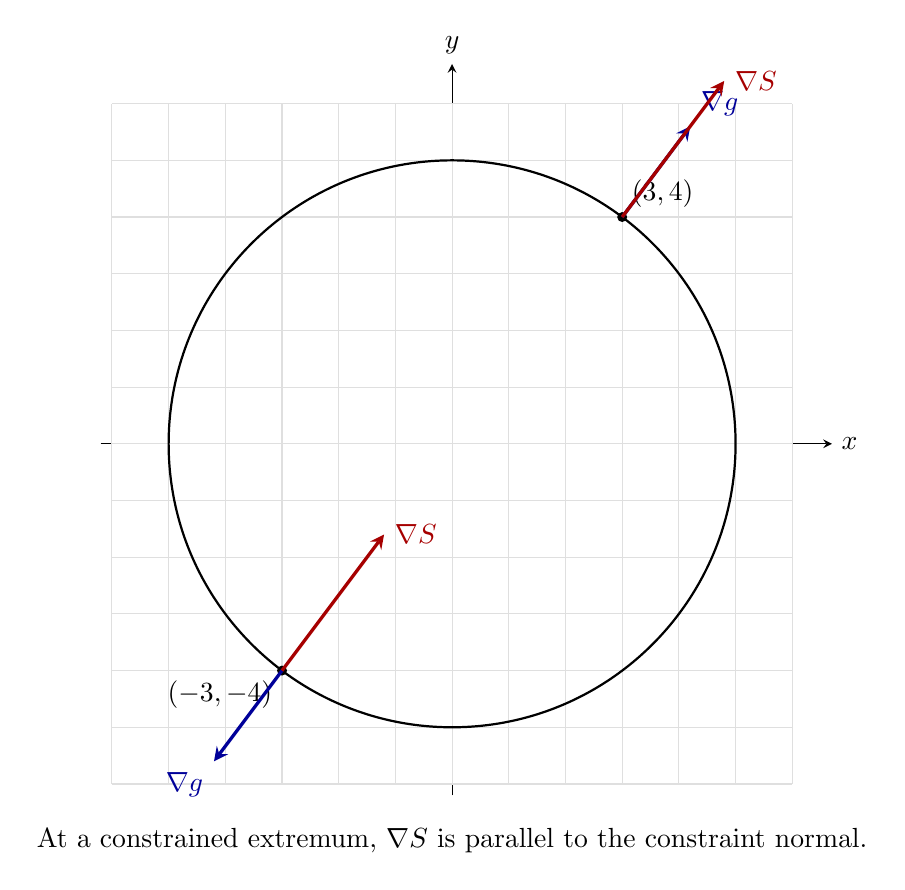
\begin{tikzpicture}[scale=0.72, >=stealth]
    \draw[->] (-6.2,0) -- (6.7,0) node[right] {\(x\)};
    \draw[->] (0,-6.2) -- (0,6.7) node[above] {\(y\)};

    \draw[gray!25, step=1] (-6,-6) grid (6,6);
    \draw[thick] (0,0) circle (5);

    \fill (3,4) circle (2.5pt);
    \node[above right] at (3,4) {\((3,4)\)};

    \fill (-3,-4) circle (2.5pt);
    \node[below left] at (-3,-4) {\((-3,-4)\)};

    \draw[->, very thick, blue!60!black] (3,4) -- ++(1.2,1.6)
        node[above right] {\(\nabla g\)};
    \draw[->, very thick, red!65!black] (3,4) -- ++(1.8,2.4)
        node[right] {\(\nabla S\)};

    \draw[->, very thick, blue!60!black] (-3,-4) -- ++(-1.2,-1.6)
        node[below left] {\(\nabla g\)};
    \draw[->, very thick, red!65!black] (-3,-4) -- ++(1.8,2.4)
        node[right] {\(\nabla S\)};

    \node at (0,-7.0) {At a constrained extremum, \(\nabla S\) is parallel to the constraint normal.};
\end{tikzpicture}
\caption{On the circle, allowed motion is tangent to the circle.  At a constrained
maximum or minimum, the gradient of the objective is normal to the allowed motion.}
\end{figure}

The number \(\lambda\) is called a \emph{Lagrange multiplier}.  The important part is
not the number itself yet.  The important part is the geometry:
\[
    \text{gradient of objective}
    \quad
    \text{is parallel to}
    \quad
    \text{gradient of constraint}.
\]

\subsection{Why the gradient is perpendicular to a constraint}

Suppose the constraint is
\[
    g(x,y)=c.
\]
A curve
\[
    \mathbf r(t)
\]
lying on the constraint satisfies
\[
    g(\mathbf r(t))=c.
\]
Differentiating gives
\[
    \nabla g(\mathbf r(t))\cdot \mathbf r'(t)=0.
\]
So every allowed tangent direction is perpendicular to
\[
    \nabla g.
\]

Now suppose \(f\) has a local maximum or minimum while the point is forced to stay
on the constraint.  Along every allowed curve through the point, the one-variable
function
\[
    f(\mathbf r(t))
\]
has a local maximum or minimum.  Therefore
\[
    \frac{d}{dt}f(\mathbf r(t))=0
\]
at that point.  By the chain rule,
\[
    \nabla f\cdot \mathbf r'(t)=0.
\]
So \(\nabla f\) is also perpendicular to every allowed tangent direction.

If the constraint is a smooth curve in the plane, then there is one tangent line.  Two
vectors perpendicular to the same tangent line must be parallel.  Therefore
\[
    \nabla f=\lambda\nabla g.
\]

In differential-form language, the same idea is even shorter.  Allowed tangent vectors
\(\mathbf v\) satisfy
\[
    dg(\mathbf v)=0.
\]
At a constrained extremum,
\[
    df(\mathbf v)=0
\]
for every allowed tangent vector.  If \(dg\ne0\), the two \(1\)-forms have the same
kernel, so
\[
\boxed{
    df=\lambda\,dg.
}
\]
In coordinates, this is
\[
\boxed{
    \nabla f=\lambda\nabla g.
}
\]

\begin{theorem}[Lagrange multiplier condition: one constraint]
Let \(f\) and \(g\) have continuous first partial derivatives near a point
\[
    \mathbf p.
\]
Suppose \(\mathbf p\) is a local maximum or local minimum of \(f\) subject to the
constraint
\[
    g(\mathbf x)=c.
\]
Suppose also that
\[
    \nabla g(\mathbf p)\ne\mathbf 0,
\]
so the constraint is a smooth level curve or level surface near \(\mathbf p\).

Then there is a number \(\lambda\) such that
\[
\boxed{
    \nabla f(\mathbf p)=\lambda\nabla g(\mathbf p).
}
\]
Equivalently,
\[
\boxed{
    df_{\mathbf p}=\lambda\,dg_{\mathbf p}.
}
\]
\end{theorem}

\begin{proof}
At the constrained extremum, \(f\) has zero first-order change in every tangent
direction allowed by the constraint.

The allowed tangent vectors \(\mathbf v\) are the vectors satisfying
\[
    dg_{\mathbf p}(\mathbf v)=0.
\]
The extremum condition says
\[
    df_{\mathbf p}(\mathbf v)=0
\]
for all such \(\mathbf v\).  Since \(dg_{\mathbf p}\ne0\), the constraint has a well-defined
normal direction.  Thus \(df_{\mathbf p}\) must point in that same normal direction,
so
\[
    df_{\mathbf p}=\lambda\,dg_{\mathbf p}
\]
for some number \(\lambda\).  In gradient notation, this becomes
\[
    \nabla f(\mathbf p)=\lambda\nabla g(\mathbf p).
\]
\end{proof}

The condition
\[
    \nabla g(\mathbf p)\ne\mathbf 0
\]
is not a technical decoration.  If the constraint gradient vanishes, the level set may
not have an ordinary tangent direction.

\begin{example}[Why the constraint gradient must not vanish]
Let
\[
    g(x,y)=x^2+y^2.
\]
The constraint
\[
    g(x,y)=0
\]
contains only the point
\[
    (0,0).
\]
Now take
\[
    f(x,y)=x.
\]
On the constraint set, \(f\) has both a maximum and a minimum, because the constraint
set has only one point.

But
\[
    \nabla f(0,0)=(1,0),
\]
while
\[
    \nabla g(0,0)=(0,0).
\]
There is no number \(\lambda\) such that
\[
    (1,0)=\lambda(0,0).
\]
The multiplier condition fails because the constraint is singular.  The level set is not
a smooth curve near the origin.
\end{example}

\subsection{One constraint in three variables}

The same condition works for surfaces in space.

\begin{example}[Closest point on a plane]
A sensor is located at
\[
    A=(1,2,3).
\]
A flat metal sheet lies in the plane
\[
    x+2y+2z=6.
\]
We want the point on the sheet closest to the sensor.

Instead of minimizing the distance, minimize the squared distance:
\[
    f(x,y,z)=(x-1)^2+(y-2)^2+(z-3)^2.
\]
The constraint is
\[
    g(x,y,z)=x+2y+2z=6.
\]
Compute the gradients:
\[
    \nabla f=
    \bigl(2(x-1),2(y-2),2(z-3)\bigr),
\]
and
\[
    \nabla g=(1,2,2).
\]
The multiplier equation is
\[
    \nabla f=\lambda\nabla g.
\]
So
\[
    2(x-1)=\lambda,
\]
\[
    2(y-2)=2\lambda,
\]
and
\[
    2(z-3)=2\lambda.
\]
Thus
\[
    x=1+\frac{\lambda}{2},
    \qquad
    y=2+\lambda,
    \qquad
    z=3+\lambda.
\]
Use the constraint:
\[
    x+2y+2z=6.
\]
Substitute:
\[
    \left(1+\frac{\lambda}{2}\right)
    +2(2+\lambda)
    +2(3+\lambda)
    =
    6.
\]
So
\[
    11+\frac{9}{2}\lambda=6.
\]
Therefore
\[
    \lambda=-\frac{10}{9}.
\]
The closest point is
\[
    x=1-\frac59=\frac49,
\]
\[
    y=2-\frac{10}{9}=\frac89,
\]
and
\[
    z=3-\frac{10}{9}=\frac{17}{9}.
\]
So
\[
\boxed{
    P=\left(\frac49,\frac89,\frac{17}{9}\right).
}
\]

Geometrically, the vector from the sheet to the sensor is normal to the sheet.  The
Lagrange equation is just that fact written in gradient form.
\end{example}

The multiplier method gives candidates.  It does not, by itself, decide whether a
candidate is a maximum, a minimum, or something else.  In the closest-point example,
the geometry tells us the answer: distance squared from a fixed point to a plane has a
unique minimum.

\subsection{Multiple constraints}

Sometimes a point must satisfy more than one constraint.

A curve in space can be described as the intersection of two surfaces:
\[
    g(x,y,z)=c,
    \qquad
    h(x,y,z)=d.
\]
At a point on the curve, the allowed tangent direction must be perpendicular to both
\[
    \nabla g
    \qquad\text{and}\qquad
    \nabla h.
\]
So the normal plane to the curve is spanned by
\[
    \nabla g
    \quad\text{and}\quad
    \nabla h,
\]
provided these two gradients are independent.

At a constrained extremum, \(\nabla f\) must also be perpendicular to the allowed
tangent direction.  Therefore \(\nabla f\) must lie in the plane spanned by the two
constraint gradients:
\[
\boxed{
    \nabla f=\lambda\nabla g+\mu\nabla h.
}
\]

\begin{theorem}[Lagrange multiplier condition: two constraints in space]
Let \(f,g,h\) have continuous first partial derivatives near a point
\[
    \mathbf p\in\mathbb R^3.
\]
Suppose \(\mathbf p\) is a local maximum or local minimum of \(f\) subject to
\[
    g(\mathbf x)=c,
    \qquad
    h(\mathbf x)=d.
\]
Suppose also that
\[
    \nabla g(\mathbf p)
    \quad\text{and}\quad
    \nabla h(\mathbf p)
\]
are linearly independent.

Then there are numbers \(\lambda\) and \(\mu\) such that
\[
\boxed{
    \nabla f(\mathbf p)
    =
    \lambda\nabla g(\mathbf p)+\mu\nabla h(\mathbf p).
}
\]
Equivalently,
\[
\boxed{
    df_{\mathbf p}
    =
    \lambda\,dg_{\mathbf p}+\mu\,dh_{\mathbf p}.
}
\]
\end{theorem}

\begin{example}[Optimizing on a circle in space]
A sensor ring lies where the cylinder
\[
    x^2+y^2=1
\]
meets the plane
\[
    z=1.
\]
On that ring, the signal strength is
\[
    F(x,y,z)=x+2y+3z.
\]
Find the maximum and minimum signal values.

Let
\[
    g(x,y,z)=x^2+y^2,
    \qquad
    h(x,y,z)=z.
\]
The constraints are
\[
    g=1,
    \qquad
    h=1.
\]
The gradients are
\[
    \nabla F=(1,2,3),
\]
\[
    \nabla g=(2x,2y,0),
\]
and
\[
    \nabla h=(0,0,1).
\]
The multiplier equation is
\[
    (1,2,3)
    =
    \lambda(2x,2y,0)+\mu(0,0,1).
\]
So
\[
    1=2\lambda x,
\]
\[
    2=2\lambda y,
\]
and
\[
    3=\mu.
\]
Thus
\[
    x=\frac{1}{2\lambda},
    \qquad
    y=\frac{1}{\lambda}.
\]
Use
\[
    x^2+y^2=1.
\]
Then
\[
    \frac{1}{4\lambda^2}+\frac{1}{\lambda^2}=1,
\]
so
\[
    \frac{5}{4\lambda^2}=1.
\]
Therefore
\[
    \lambda=\pm\frac{\sqrt5}{2}.
\]

When
\[
    \lambda=\frac{\sqrt5}{2},
\]
we get
\[
    x=\frac{1}{\sqrt5},
    \qquad
    y=\frac{2}{\sqrt5},
    \qquad
    z=1.
\]
When
\[
    \lambda=-\frac{\sqrt5}{2},
\]
we get
\[
    x=-\frac{1}{\sqrt5},
    \qquad
    y=-\frac{2}{\sqrt5},
    \qquad
    z=1.
\]

The corresponding values are
\[
    F\left(\frac{1}{\sqrt5},\frac{2}{\sqrt5},1\right)
    =
    \frac{1}{\sqrt5}+\frac{4}{\sqrt5}+3
    =
    3+\sqrt5,
\]
and
\[
    F\left(-\frac{1}{\sqrt5},-\frac{2}{\sqrt5},1\right)
    =
    3-\sqrt5.
\]
The ring is closed and bounded, so a continuous function on it has an absolute maximum
and minimum.  Thus
\[
\boxed{
    \text{maximum value }3+\sqrt5
}
\]
and
\[
\boxed{
    \text{minimum value }3-\sqrt5.
}
\]
\end{example}

\subsection{Boundary constraints and compactness}

Lagrange multipliers find candidates on smooth constraint pieces.  Boundary points
must still be checked separately.

The guiding theorem is the same extreme-value theorem from single-variable calculus,
now used in the plane and in space.

\begin{theorem}[Extreme-value theorem]
Let \(D\) be a closed and bounded set in \(\mathbb R^2\) or \(\mathbb R^3\).  If
\[
    f:D\to\mathbb R
\]
is continuous, then \(f\) attains an absolute maximum and an absolute minimum on
\(D\).
\end{theorem}

Here \emph{closed and bounded} is the practical meaning of compact in the spaces of
this book.  Closed means the boundary is included.  Bounded means the set fits inside
some large ball.

Each hypothesis matters.

\begin{example}[Why closed matters]
The function
\[
    f(x)=x
\]
on the open interval
\[
    0<x<1
\]
has no maximum and no minimum.  The values get close to \(1\) and close to \(0\),
but the endpoints are missing.
\end{example}

\begin{example}[Why bounded matters]
The function
\[
    f(x)=x
\]
on the real line has no maximum and no minimum.  The domain is closed, but it is
not bounded.
\end{example}

\begin{example}[Why continuity matters]
Define
\[
    f(x)=
    \begin{cases}
    \dfrac1x, & 0<x\le1,\\[2mm]
    0, & x=0.
    \end{cases}
\]
The domain
\[
    [0,1]
\]
is closed and bounded.  But \(f\) is not continuous at \(0\), and it has no maximum:
as \(x\to0^+\), the values
\[
    \frac1x
\]
grow without bound.
\end{example}

For practical optimization on a region, the candidate list usually has several parts:

\[
\begin{array}{c|l}
\text{Place} & \text{What to do}\\ \hline
\text{interior} & \nabla f=\mathbf 0\\[1mm]
\text{smooth boundary pieces} & \text{use Lagrange multipliers or one-variable calculus}\\[1mm]
\text{corners and endpoints} & \text{check directly}
\end{array}
\]

\begin{example}[A semicircular courtyard]
A solar sensor can be placed anywhere in the upper half-disk
\[
    D=\{(x,y):x^2+y^2\le25,\ y\ge0\}.
\]
Its score is
\[
    S(x,y)=6x+8y.
\]
Find the absolute maximum and minimum.

The domain is closed and bounded, and \(S\) is continuous.  Therefore the absolute
maximum and minimum exist.

There are no interior critical points, because
\[
    \nabla S=(6,8)\ne\mathbf 0.
\]

Now check the curved boundary
\[
    x^2+y^2=25,
    \qquad
    y\ge0.
\]
Using
\[
    g(x,y)=x^2+y^2,
\]
the multiplier equation is
\[
    (6,8)=\lambda(2x,2y).
\]
As before, this gives
\[
    (x,y)=(3,4)
    \qquad\text{or}\qquad
    (x,y)=(-3,-4).
\]
Only
\[
    (3,4)
\]
lies on the upper semicircle.

Now check the flat boundary
\[
    y=0,
    \qquad
    -5\le x\le5.
\]
There
\[
    S(x,0)=6x.
\]
On the interval \([-5,5]\), this has endpoint values
\[
    S(5,0)=30,
    \qquad
    S(-5,0)=-30.
\]

Compare the candidates:
\[
    S(3,4)=50,
\]
\[
    S(5,0)=30,
\]
and
\[
    S(-5,0)=-30.
\]
Therefore
\[
\boxed{
    \text{absolute maximum }50\text{ at }(3,4),
}
\]
and
\[
\boxed{
    \text{absolute minimum }-30\text{ at }(-5,0).
}
\]

The minimum occurs at an endpoint of a boundary piece.  It is not found by the smooth
circle multiplier equation.
\end{example}

\subsection{Interpreting the multiplier}

The multiplier \(\lambda\) often has a useful meaning.  It measures how the best value
changes when the constraint level changes.

Return to the circular path problem:
\[
    S(x,y)=6x+8y,
    \qquad
    x^2+y^2=25.
\]
More generally, suppose the constraint is
\[
    x^2+y^2=c,
\]
where \(c>0\).  This is a circle of radius
\[
    \sqrt c.
\]
The maximum of \(S\) on that circle is
\[
    M(c)=10\sqrt c,
\]
because the vector \((6,8)\) has length \(10\).

Differentiate:
\[
    M'(c)=\frac{5}{\sqrt c}.
\]
At
\[
    c=25,
\]
we get
\[
    M'(25)=1.
\]
That matches the multiplier at the maximum point \((3,4)\), where
\[
    \lambda=1.
\]

So if the allowed squared radius \(c\) increases slightly, the maximum sunlight score
increases by about
\[
    1
\]
unit of score per unit of \(c\).

The unit matters.  If instead we write the constraint as
\[
    \sqrt{x^2+y^2}=R,
\]
then the maximum value is
\[
    10R.
\]
At
\[
    R=5,
\]
its derivative is
\[
    10.
\]
The multiplier changes because the constraint parameter changed.  One version measures
change per unit of squared radius.  The other measures change per unit of radius.

This is one reason Lagrange multipliers appear in economics, physics, and design
problems.  They do not only find candidates.  They also tell how valuable it would be
to relax a constraint.  But the method is easy to over-trust.  It speaks only under its
hypotheses, and it speaks only about the pieces where those hypotheses hold.  The next
section collects the traps, because most wrong optimization solutions fail in exactly
these places.

\section{Warning examples}
\label{sec:9.6}

The tests in this chapter are powerful because they are conditional.  They say:

\[
    \text{if the hypotheses hold, then the conclusion follows.}
\]

A warning example shows what can happen when one of the hypotheses is missing, or
when a test is used beyond what it says.

\subsection{A critical point that is not an extremum}

The equation
\[
    \nabla f=\mathbf 0
\]
does not mean maximum or minimum.  It means first-order silence.

Let
\[
    f(x,y)=x^2-y^2.
\]
Then
\[
    f_x=2x,
    \qquad
    f_y=-2y.
\]
So
\[
    \nabla f(0,0)=\mathbf 0.
\]
The origin is a critical point.

But along the \(x\)-axis,
\[
    f(x,0)=x^2>0
\]
for \(x\ne0\).  Along the \(y\)-axis,
\[
    f(0,y)=-y^2<0
\]
for \(y\ne0\).

Thus every small disk around the origin contains points where \(f\) is larger than
\(f(0,0)\) and points where \(f\) is smaller.  The origin is a saddle point.

The gradient equation finds candidates.  It does not classify them.

\subsection{A degenerate Hessian with a minimum}

The second derivative test also has limits.  If the Hessian is degenerate, second-order
information may not decide the shape.

Let
\[
    f(x,y)=x^4+y^4.
\]
Then
\[
    \nabla f(x,y)=(4x^3,4y^3),
\]
so
\[
    \nabla f(0,0)=\mathbf 0.
\]
The Hessian is
\[
    H_f(x,y)
    =
    \begin{pmatrix}
        12x^2 & 0\\
        0 & 12y^2
    \end{pmatrix}.
\]
At the origin,
\[
    H_f(0,0)
    =
    \begin{pmatrix}
        0&0\\
        0&0
    \end{pmatrix}.
\]
So
\[
    \Delta=0.
\]
The second derivative test gives no conclusion.

But
\[
    x^4+y^4\ge0
\]
for all \((x,y)\), with equality only at
\[
    (0,0).
\]
Therefore the origin is a local minimum.

Here the first nonzero visible terms are fourth order, not second order.

\subsection{A degenerate Hessian with a saddle point}

Now change only one sign:
\[
    g(x,y)=x^4-y^4.
\]
Again
\[
    \nabla g(0,0)=\mathbf 0,
\]
and again
\[
    H_g(0,0)
    =
    \begin{pmatrix}
        0&0\\
        0&0
    \end{pmatrix}.
\]
The Hessian at the origin is exactly the same as in the previous example.

But along the \(x\)-axis,
\[
    g(t,0)=t^4>0
\]
for \(t\ne0\), while along the \(y\)-axis,
\[
    g(0,t)=-t^4<0
\]
for \(t\ne0\).

So the origin is a saddle point.

The same degenerate Hessian led to a minimum in one example and a saddle point in
the other.  When
\[
    \Delta=0,
\]
the second derivative test is not weak.  It is honest: second-order information is not
enough.

\subsection{A constrained problem where the multiplier method misses an endpoint}

Lagrange multipliers are for smooth constraint pieces.  They do not automatically find
endpoints or corners.

Find the maximum and minimum of
\[
    f(x,y)=x
\]
on the line segment
\[
    -1\le x\le1,
    \qquad
    y=0.
\]
The smooth constraint is
\[
    g(x,y)=y=0.
\]
Then
\[
    \nabla f=(1,0),
    \qquad
    \nabla g=(0,1).
\]
The multiplier equation would be
\[
    (1,0)=\lambda(0,1),
\]
which has no solution.

That does not mean the problem has no extrema.  The domain is the closed line segment.
The maximum occurs at
\[
    (1,0),
\]
and the minimum occurs at
\[
    (-1,0).
\]

The multiplier method found no interior point of the segment because the function is
increasing all along the segment.  The extrema live at the endpoints, where the allowed
set stops.

\subsection{Mixed partials can fail to agree without regularity}

For smooth functions, the mixed partials agree:
\[
    f_{xy}=f_{yx}.
\]
But the continuity hypothesis in the mixed-partials theorem is not optional.

Define
\[
    F(x,y)=
    \begin{cases}
    \dfrac{xy(x^2-y^2)}{x^2+y^2}, & (x,y)\ne(0,0),\\[3mm]
    0, & (x,y)=(0,0).
    \end{cases}
\]
At the origin, compute the mixed partials by looking along the axes.

First, for \(y\ne0\),
\[
\begin{aligned}
F_x(0,y)
&=
\lim_{h\to0}
\frac{F(h,y)-F(0,y)}{h}\\
&=
\lim_{h\to0}
\frac{hy(h^2-y^2)}{h(h^2+y^2)}\\
&=
\lim_{h\to0}
\frac{y(h^2-y^2)}{h^2+y^2}\\
&=
-y.
\end{aligned}
\]
Also \(F_x(0,0)=0\), so near the origin along the \(y\)-axis,
\[
    F_x(0,y)=-y.
\]
Therefore
\[
    F_{xy}(0,0)
    =
    \lim_{k\to0}
    \frac{F_x(0,k)-F_x(0,0)}{k}
    =
    \lim_{k\to0}
    \frac{-k}{k}
    =
    -1.
\]

Now reverse the order.  For \(x\ne0\),
\[
\begin{aligned}
F_y(x,0)
&=
\lim_{k\to0}
\frac{F(x,k)-F(x,0)}{k}\\
&=
\lim_{k\to0}
\frac{xk(x^2-k^2)}{k(x^2+k^2)}\\
&=
\lim_{k\to0}
\frac{x(x^2-k^2)}{x^2+k^2}\\
&=
x.
\end{aligned}
\]
Also \(F_y(0,0)=0\), so near the origin along the \(x\)-axis,
\[
    F_y(x,0)=x.
\]
Therefore
\[
    F_{yx}(0,0)
    =
    \lim_{h\to0}
    \frac{F_y(h,0)-F_y(0,0)}{h}
    =
    \lim_{h\to0}
    \frac{h}{h}
    =
    1.
\]

So
\[
\boxed{
    F_{xy}(0,0)=-1,
    \qquad
    F_{yx}(0,0)=1.
}
\]
Both mixed partials exist at the origin, but they are not equal.  The missing condition
is regularity near the point, such as continuity of the mixed partials.

\subsection{The common lesson}

The warnings are different, but they share one pattern.

\[
\begin{array}{c|l}
\text{Tool} & \text{What it does not do}\\ \hline
\nabla f=\mathbf 0 & \text{does not guarantee an extremum}\\[1mm]
\text{second derivative test} & \text{does not classify degenerate Hessians}\\[1mm]
\text{Lagrange multipliers} & \text{does not check endpoints, corners, or singular constraints}\\[1mm]
f_{xy}=f_{yx} & \text{does not hold without enough regularity}
\end{array}
\]

This chapter has been about special points: peaks, valleys, saddles, and constrained
extrema.  The next chapter changes the question.  Instead of asking where a function is
largest or smallest, we will ask how to add its values over a whole region.  A hill will
no longer be judged by its highest point, but by the total amount of earth under it.  That
new operation is the double integral.
% =====================================================================
%  Chapter 9: Gradients, Hessians, and Optimization
%  Section 9.7
% =====================================================================

\section{Chapter review and applications}
\label{sec:9.7}

Section \ref{sec:9.6} collected the traps.  A zero gradient may hide a saddle.  A
degenerate Hessian may hide higher-order behavior.  A Lagrange multiplier calculation
may miss an endpoint.  Those warnings do not weaken the tools.  They tell us where
each tool belongs.

This review gathers the chapter into one decision path.

\subsection{The chapter in one picture}

Optimization begins by asking what motions are allowed.

If a point is free to move in every direction, then an interior extremum forces
\[
    df=\mathbf 0,
\]
or, in gradient notation,
\[
    \nabla f=\mathbf 0.
\]
If the point must stay on a constraint
\[
    g=c,
\]
then only tangent directions to the constraint are allowed.  At a constrained extremum,
\[
    df=\lambda\,dg,
\]
or
\[
    \nabla f=\lambda\nabla g.
\]

After first-order candidates are found, the Hessian reads the second-order shape.

\begin{figure}[h]
\centering
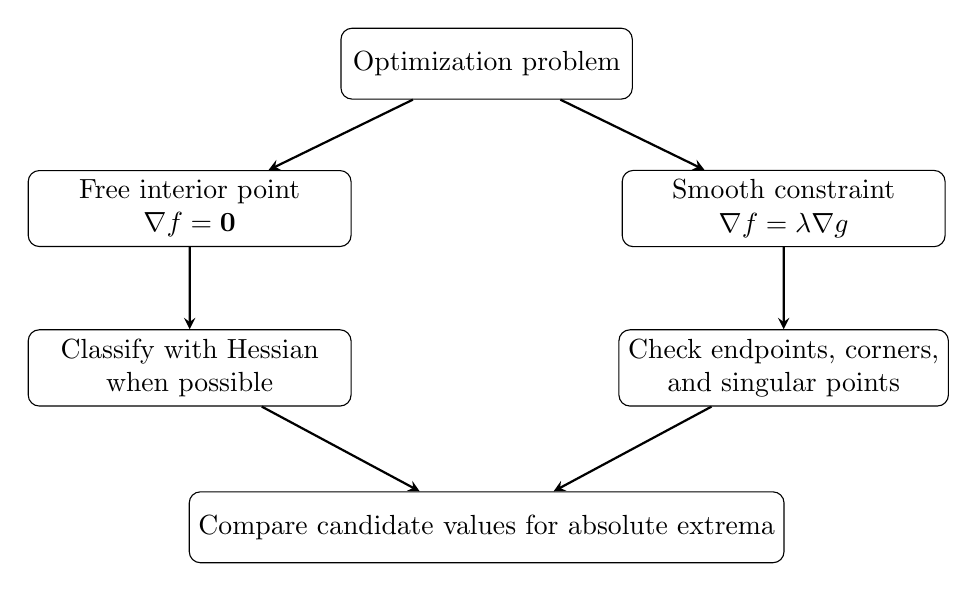
\begin{tikzpicture}[scale=0.92, >=stealth]
    \node[draw, rounded corners, align=center, minimum width=3.7cm, minimum height=0.9cm]
        (start) at (0,0) {Optimization problem};

    \node[draw, rounded corners, align=center, minimum width=4.1cm, minimum height=0.9cm]
        (free) at (-4.1,-2) {Free interior point\\ \(\nabla f=\mathbf 0\)};

    \node[draw, rounded corners, align=center, minimum width=4.1cm, minimum height=0.9cm]
        (constr) at (4.1,-2) {Smooth constraint\\ \(\nabla f=\lambda\nabla g\)};

    \node[draw, rounded corners, align=center, minimum width=4.1cm, minimum height=0.9cm]
        (hess) at (-4.1,-4.2) {Classify with Hessian\\ when possible};

    \node[draw, rounded corners, align=center, minimum width=4.1cm, minimum height=0.9cm]
        (boundary) at (4.1,-4.2) {Check endpoints, corners,\\ and singular points};

    \node[draw, rounded corners, align=center, minimum width=5.3cm, minimum height=0.9cm]
        (compare) at (0,-6.4) {Compare candidate values for absolute extrema};

    \draw[->, thick] (start) -- (free);
    \draw[->, thick] (start) -- (constr);
    \draw[->, thick] (free) -- (hess);
    \draw[->, thick] (constr) -- (boundary);
    \draw[->, thick] (hess) -- (compare);
    \draw[->, thick] (boundary) -- (compare);
\end{tikzpicture}
\caption{The first question is not ``Which formula do I use?'' but ``What motions are
allowed?''}
\end{figure}

The main tests can be kept in one table.

\[
\begin{array}{c|c|c}
\text{Situation} & \text{Candidate condition} & \text{What to do next} \\ \hline
\text{free interior point}
&
\nabla f=\mathbf 0
&
\text{use Hessian if second derivatives behave well}
\\[2mm]
\text{derivative fails}
&
\text{point is still a candidate}
&
\text{check directly}
\\[2mm]
\text{boundary point}
&
\text{ordinary }\nabla f=\mathbf 0\text{ may fail}
&
\text{optimize on the boundary}
\\[2mm]
\text{smooth constraint }g=c
&
\nabla f=\lambda\nabla g
&
\text{compare constrained candidates}
\\[2mm]
\text{two constraints}
&
\nabla f=\lambda\nabla g+\mu\nabla h
&
\text{compare constrained candidates}
\end{array}
\]

For a twice continuously differentiable function of two variables, the Hessian test at a
critical point uses
\[
    A=f_{xx},
    \qquad
    B=f_{xy},
    \qquad
    C=f_{yy},
\]
and
\[
    \Delta=AC-B^2.
\]

\[
\begin{array}{c|c}
\text{Condition} & \text{Conclusion} \\ \hline
\Delta>0,\ A>0 & \text{local minimum}\\[1mm]
\Delta>0,\ A<0 & \text{local maximum}\\[1mm]
\Delta<0 & \text{saddle point}\\[1mm]
\Delta=0 & \text{test gives no conclusion}
\end{array}
\]

The number
\[
    \Delta
\]
is only reading the quadratic part.  If the quadratic part is silent in some direction, the
function may still be decided by third, fourth, or higher-order terms.

\subsection{Worked review example: free critical points}

Let
\[
    f(x,y)=x^3-3x+y^2-4y.
\]
Find and classify the critical points.

First compute the gradient:
\[
    f_x=3x^2-3,
    \qquad
    f_y=2y-4.
\]
Set both equal to zero:
\[
    3x^2-3=0,
    \qquad
    2y-4=0.
\]
Thus
\[
    x=\pm1,
    \qquad
    y=2.
\]
The critical points are
\[
    (1,2)
    \qquad\text{and}\qquad
    (-1,2).
\]

Now compute the second partials:
\[
    f_{xx}=6x,
    \qquad
    f_{xy}=0,
    \qquad
    f_{yy}=2.
\]

At
\[
    (1,2),
\]
we have
\[
    A=6,\qquad B=0,\qquad C=2.
\]
So
\[
    \Delta=AC-B^2=12>0,
\]
and
\[
    A>0.
\]
Therefore
\[
\boxed{
    (1,2)\text{ is a local minimum.}
}
\]

At
\[
    (-1,2),
\]
we have
\[
    A=-6,\qquad B=0,\qquad C=2.
\]
So
\[
    \Delta=(-6)(2)-0=-12<0.
\]
Therefore
\[
\boxed{
    (-1,2)\text{ is a saddle point.}
}
\]

The same function has both behaviors.  The gradient found the silent points.  The
Hessian listened to the first nonzero shape near each one.

\subsection{Worked review example: absolute extrema on a rectangle}

Let
\[
    f(x,y)=x^2+2y^2-4x-4y
\]
on the rectangle
\[
    0\le x\le 3,
    \qquad
    0\le y\le 2.
\]
Find the absolute maximum and minimum.

The domain is closed and bounded, and \(f\) is continuous, so an absolute maximum and
minimum exist.

First check the interior.  The gradient is
\[
    \nabla f=(2x-4,\;4y-4).
\]
Set it equal to zero:
\[
    2x-4=0,
    \qquad
    4y-4=0.
\]
Thus
\[
    x=2,
    \qquad
    y=1.
\]
This point lies inside the rectangle.  Its value is
\[
    f(2,1)=4+2-8-4=-6.
\]

Now check the boundary.

On the left edge,
\[
    x=0,\qquad 0\le y\le2.
\]
Then
\[
    f(0,y)=2y^2-4y=2(y-1)^2-2.
\]
The minimum on this edge is \(-2\), and the maximum is \(0\), reached at
\[
    y=0
    \qquad\text{and}\qquad
    y=2.
\]

On the right edge,
\[
    x=3,\qquad 0\le y\le2.
\]
Then
\[
    f(3,y)=9+2y^2-12-4y=2(y-1)^2-5.
\]
The minimum on this edge is \(-5\), and the maximum is \(-3\).

On the bottom edge,
\[
    y=0,\qquad 0\le x\le3.
\]
Then
\[
    f(x,0)=x^2-4x=(x-2)^2-4.
\]
The minimum on this edge is \(-4\), and the maximum is \(0\), reached at \(x=0\).

On the top edge,
\[
    y=2,\qquad 0\le x\le3.
\]
Then
\[
    f(x,2)=x^2+8-4x-8=x^2-4x=(x-2)^2-4.
\]
The minimum on this edge is \(-4\), and the maximum is \(0\), reached at \(x=0\).

Compare all candidates:
\[
\begin{array}{c|c}
\text{candidate} & f(x,y) \\ \hline
(2,1) & -6\\
(0,0) & 0\\
(0,2) & 0\\
\text{other boundary candidates} & -5,\,-4,\,-3,\,-2
\end{array}
\]

Therefore
\[
\boxed{
    \text{absolute minimum }-6\text{ at }(2,1),
}
\]
and
\[
\boxed{
    \text{absolute maximum }0\text{ at }(0,0)\text{ and }(0,2).
}
\]

The interior gradient found the minimum.  The maximum lived on the boundary.

\subsection{Worked review example: one smooth constraint}

Find the maximum and minimum of
\[
    p(x,y)=x+2y
\]
on the ellipse
\[
    x^2+4y^2=16.
\]

Let
\[
    g(x,y)=x^2+4y^2.
\]
The constraint is
\[
    g=16.
\]
The gradients are
\[
    \nabla p=(1,2),
    \qquad
    \nabla g=(2x,8y).
\]
The Lagrange multiplier equation is
\[
    \nabla p=\lambda\nabla g.
\]
So
\[
    1=2\lambda x,
    \qquad
    2=8\lambda y.
\]
Thus
\[
    x=\frac{1}{2\lambda},
    \qquad
    y=\frac{1}{4\lambda}.
\]
Substitute into the constraint:
\[
    x^2+4y^2=16.
\]
This gives
\[
    \frac{1}{4\lambda^2}
    +
    4\cdot\frac{1}{16\lambda^2}
    =
    16,
\]
so
\[
    \frac{1}{2\lambda^2}=16.
\]
Therefore
\[
    \lambda^2=\frac{1}{32},
\]
and
\[
    \lambda=\pm \frac{1}{4\sqrt2}.
\]

When
\[
    \lambda=\frac{1}{4\sqrt2},
\]
we get
\[
    x=2\sqrt2,
    \qquad
    y=\sqrt2.
\]
When
\[
    \lambda=-\frac{1}{4\sqrt2},
\]
we get
\[
    x=-2\sqrt2,
    \qquad
    y=-\sqrt2.
\]

The values are
\[
    p(2\sqrt2,\sqrt2)=2\sqrt2+2\sqrt2=4\sqrt2,
\]
and
\[
    p(-2\sqrt2,-\sqrt2)=-4\sqrt2.
\]
The ellipse is closed and bounded, so these are the absolute extrema:
\[
\boxed{
    \text{maximum }4\sqrt2\text{ at }(2\sqrt2,\sqrt2),
}
\]
\[
\boxed{
    \text{minimum }-4\sqrt2\text{ at }(-2\sqrt2,-\sqrt2).
}
\]

Geometrically, the level lines
\[
    x+2y=c
\]
slide across the ellipse.  At the largest and smallest values, the line just touches the
ellipse.  At those touching points, the normal direction to the line is parallel to the
normal direction to the ellipse.

\subsection{Concept check}

\begin{enumerate}
\item Why is the gradient normal to a level curve?

\item What is the tangent line to
\[
    f(x,y)=f(a,b)
\]
at a point where
\[
    \nabla f(a,b)\ne\mathbf 0?
\]

\item What is the tangent plane to
\[
    F(x,y,z)=F(a,b,c)
\]
at a point where
\[
    \nabla F(a,b,c)\ne\mathbf 0?
\]

\item Why must an interior local maximum or minimum of a differentiable function
satisfy
\[
    \nabla f=\mathbf 0?
\]

\item Why does
\[
    \nabla f=\mathbf 0
\]
not guarantee a maximum or minimum?

\item What information does the Hessian contain that the gradient does not?

\item In the two-variable second derivative test, what does
\[
    \Delta=f_{xx}f_{yy}-f_{xy}^2
\]
measure?

\item What does it mean for a Hessian to be positive definite?  What local shape does
that suggest at a critical point?

\item Why does the second derivative test require the point to be critical?

\item Why does the test give no conclusion when
\[
    \Delta=0?
\]

\item Why does a constrained extremum usually satisfy
\[
    \nabla f=\lambda\nabla g
\]
instead of
\[
    \nabla f=\mathbf 0?
\]

\item What can go wrong if
\[
    \nabla g=\mathbf 0
\]
on the constraint?

\item Why must endpoints and corners be checked separately?

\item In the differential-form notation
\[
    df=\lambda\,dg,
\]
what does the equation say about allowed tangent motions?
\end{enumerate}

\subsection{Skill problems}

\begin{enumerate}
\item Let
\[
    f(x,y)=x^2+xy+y^2.
\]
Find the tangent line to the level curve
\[
    f(x,y)=3
\]
at
\[
    (1,1).
\]

\item Let
\[
    F(x,y,z)=x^2+2y^2+3z^2.
\]
Find the tangent plane to
\[
    F(x,y,z)=9
\]
at
\[
    (1,1,\sqrt2).
\]

\item Let
\[
    h(x,y)=20+4x-y-x^2-2y^2.
\]
Find all critical points and classify them.

\item Let
\[
    f(x,y)=x^3-3x+y^2-2y.
\]
Find all critical points and classify them.

\item Let
\[
    q(x,y)=x^2+4xy+y^2.
\]
Classify the origin using the Hessian.

\item Let
\[
    s(x,y)=x^2+xy+2y^2.
\]
Use the Hessian to decide whether the origin is a local maximum, local minimum, or
saddle point.

\item Let
\[
    f(x,y)=x^4+y^2.
\]
Explain why the second derivative test gives no conclusion at the origin, and then
classify the origin directly.

\item Let
\[
    g(x,y)=x^4-y^2.
\]
Explain why the origin is a saddle point even though the Hessian is degenerate.

\item Find the absolute maximum and minimum of
\[
    f(x,y)=x+y
\]
on the closed disk
\[
    x^2+y^2\le 9.
\]

\item Find the absolute maximum and minimum of
\[
    f(x,y)=x^2+y^2-2x
\]
on the rectangle
\[
    -1\le x\le3,
    \qquad
    0\le y\le2.
\]

\item Use Lagrange multipliers to find the maximum and minimum of
\[
    f(x,y)=3x+4y
\]
on the circle
\[
    x^2+y^2=25.
\]

\item Use Lagrange multipliers to find the maximum and minimum of
\[
    f(x,y)=xy
\]
on the ellipse
\[
    x^2+4y^2=16.
\]

\item Find the point on the plane
\[
    x+y+z=6
\]
closest to the origin.

\item Find the point on the sphere
\[
    x^2+y^2+z^2=25
\]
where
\[
    f(x,y,z)=x+2y+2z
\]
is largest.

\item Find the maximum and minimum of
\[
    f(x,y,z)=z
\]
on the curve where
\[
    x^2+y^2+z^2=9,
    \qquad
    x+y=0.
\]

\item Let
\[
    f(x,y)=x^2+y^2
\]
subject to
\[
    y=x^2.
\]
Find the constrained critical points by reducing to one variable.  Then explain why the
ordinary condition
\[
    \nabla f=\lambda\nabla g
\]
must be used with care at singular constraints.

\item Let
\[
    f(x,y)=x
\]
on the line segment
\[
    -1\le x\le1,
    \qquad
    y=0.
\]
Explain why the Lagrange multiplier equation for the smooth line \(y=0\) finds no
candidate, even though the function has a maximum and a minimum on the segment.

\item Let
\[
    f(x,y)=|x|+y^2.
\]
Does \(f\) have a local minimum at the origin?  Is the gradient defined there?

\item Let
\[
    f(x,y)=x^2-y^2+x^4.
\]
Classify the origin.

\item Let
\[
    f(x,y)=x^4+y^4-4xy.
\]
Find all critical points.  Use the Hessian where possible.

\item Let
\[
    f(x,y)=e^{x+y}(x^2+y^2).
\]
Show that the origin is a critical point and classify it.

\item Let
\[
    f(x,y)=x^2+2y^2+2xy-6x.
\]
Complete the square to classify its critical point.  Then check your answer with the
Hessian.

\item Let
\[
    F(x,y)=
    \begin{cases}
    \dfrac{xy(x^2-y^2)}{x^2+y^2}, & (x,y)\ne(0,0),\\[3mm]
    0, & (x,y)=(0,0).
    \end{cases}
\]
Compute
\[
    F_{xy}(0,0)
    \qquad\text{and}\qquad
    F_{yx}(0,0).
\]
What hypothesis of the mixed-partials theorem fails?

\item Give an example of a critical point where the Hessian is the zero matrix but the
point is a local minimum.

\item Give an example of a critical point where the Hessian is the zero matrix but the
point is a saddle point.
\end{enumerate}

\subsection{Discovery project: least squares and the geometry of best fit}

A line rarely passes exactly through experimental data.  Suppose a lab records four
points:
\[
    (0,1),\qquad (1,2),\qquad (2,2),\qquad (3,4).
\]
We want a line
\[
    y=mx+b
\]
that fits them as well as possible.

For each data point \((x_i,y_i)\), the vertical error is
\[
    mx_i+b-y_i.
\]
Instead of minimizing the sum of errors, which can cancel positive and negative
mistakes, minimize the sum of squared errors:
\[
\boxed{
    E(m,b)=\sum_{i=1}^4(mx_i+b-y_i)^2.
}
\]
For these data,
\[
\boxed{
    E(m,b)
    =
    (b-1)^2+(m+b-2)^2+(2m+b-2)^2+(3m+b-4)^2.
}
\]

The best-fit line is found by minimizing \(E\).  This is an optimization problem in the
two variables
\[
    m
    \qquad\text{and}\qquad
    b.
\]

\subsubsection*{Part 1. The normal equations}

Differentiate:
\[
    E_m=2\sum_{i=1}^4 x_i(mx_i+b-y_i),
\]
and
\[
    E_b=2\sum_{i=1}^4 (mx_i+b-y_i).
\]
At the minimum,
\[
    E_m=0,
    \qquad
    E_b=0.
\]
These are called the normal equations.

For the four data points, compute
\[
    \sum x_i=6,
    \qquad
    \sum x_i^2=14,
    \qquad
    \sum y_i=9,
    \qquad
    \sum x_iy_i=18.
\]
Show that the equations become
\[
\boxed{
    14m+6b=18,
}
\]
and
\[
\boxed{
    6m+4b=9.
}
\]
Solve them to get
\[
\boxed{
    m=\frac{9}{10},
    \qquad
    b=\frac{9}{10}.
}
\]
So the least-squares line is
\[
\boxed{
    y=\frac{9}{10}x+\frac{9}{10}.
}
\]

\subsubsection*{Part 2. Why this critical point is a minimum}

The Hessian of \(E\) is
\[
    H_E
    =
    2
    \begin{pmatrix}
        \sum x_i^2 & \sum x_i\\
        \sum x_i & 4
    \end{pmatrix}
    =
    \begin{pmatrix}
        28 & 12\\
        12 & 8
    \end{pmatrix}.
\]
Compute
\[
    \Delta=28\cdot8-12^2=224-144=80>0.
\]
Since
\[
    A=28>0,
\]
the Hessian is positive definite.  Therefore the critical point is a local minimum.

Because \(E(m,b)\) is a quadratic function whose leading quadratic part is positive
definite, this local minimum is the absolute minimum.

\subsubsection*{Part 3. The geometry of the residual}

Let
\[
    \mathbf y=(1,2,2,4)
\]
be the vector of measured \(y\)-values.  Let
\[
    \mathbf 1=(1,1,1,1),
    \qquad
    \mathbf x=(0,1,2,3).
\]
The predicted values from the line
\[
    y=mx+b
\]
form the vector
\[
    \widehat{\mathbf y}=m\mathbf x+b\mathbf 1.
\]
The residual vector is
\[
    \mathbf r=\widehat{\mathbf y}-\mathbf y.
\]

At the best-fit line,
\[
    m=b=\frac9{10}.
\]
So
\[
    \widehat{\mathbf y}
    =
    \left(\frac9{10},\frac{18}{10},\frac{27}{10},\frac{36}{10}\right),
\]
and
\[
    \mathbf r
    =
    \left(-\frac1{10},-\frac2{10},\frac7{10},-\frac4{10}\right).
\]
Check that
\[
\boxed{
    \mathbf r\cdot \mathbf 1=0
}
\]
and
\[
\boxed{
    \mathbf r\cdot \mathbf x=0.
}
\]

The residual is perpendicular to every change caused by adjusting \(b\) or adjusting
\(m\).  This is the geometric meaning of the normal equations: the error left over is
orthogonal to the space of possible predictions.

\subsubsection*{What to hand in}

Write a short report with the following pieces.

\begin{enumerate}
\item A plot of the four data points and the best-fit line.

\item The error function
\[
    E(m,b).
\]

\item The two normal equations
\[
    E_m=0,\qquad E_b=0.
\]

\item The solution
\[
    m=b=\frac9{10}.
\]

\item The Hessian calculation showing that this point gives a minimum.

\item The residual vector and the two dot products
\[
    \mathbf r\cdot\mathbf 1=0,
    \qquad
    \mathbf r\cdot\mathbf x=0.
\]

\item A paragraph explaining why ``best fit'' means a perpendicular residual.
\end{enumerate}

\subsection{Discovery project: designing a container under constraints}

A rectangular open-top container has base side lengths
\[
    x,\qquad y
\]
and height
\[
    z.
\]
It must have volume
\[
    32
\]
cubic units:
\[
    xyz=32.
\]
The amount of material needed is
\[
    A(x,y,z)=xy+2xz+2yz.
\]
The term \(xy\) is the base.  The terms \(2xz\) and \(2yz\) are the four side walls.
There is no top.

Find the dimensions that use the least material.

\subsubsection*{Part 1. Set up the Lagrange equations}

Let
\[
    g(x,y,z)=xyz.
\]
The constraint is
\[
    g=32.
\]
The gradients are
\[
    \nabla A=(y+2z,\ x+2z,\ 2x+2y),
\]
and
\[
    \nabla g=(yz,\ xz,\ xy).
\]
The Lagrange multiplier equation is
\[
    \nabla A=\lambda\nabla g.
\]
So
\[
    y+2z=\lambda yz,
\]
\[
    x+2z=\lambda xz,
\]
\[
    2x+2y=\lambda xy,
\]
together with
\[
    xyz=32.
\]

\subsubsection*{Part 2. Show that the base is square}

Multiply the first equation by \(x\):
\[
    xy+2xz=\lambda xyz.
\]
Multiply the second equation by \(y\):
\[
    xy+2yz=\lambda xyz.
\]
Subtract:
\[
    2xz-2yz=0.
\]
Since
\[
    z>0,
\]
we get
\[
\boxed{
    x=y.
}
\]

Set
\[
    x=y=a.
\]
The third Lagrange equation becomes
\[
    4a=\lambda a^2,
\]
so
\[
    \lambda=\frac4a.
\]
The first equation becomes
\[
    a+2z=\lambda az.
\]
Substitute
\[
    \lambda=\frac4a:
\]
\[
    a+2z=4z.
\]
Therefore
\[
\boxed{
    a=2z.
}
\]
So
\[
    z=\frac a2.
\]

Use the volume constraint:
\[
    a^2z=32.
\]
Since
\[
    z=\frac a2,
\]
we get
\[
    a^2\cdot\frac a2=32,
\]
so
\[
    a^3=64.
\]
Thus
\[
    a=4,
\]
and
\[
    z=2.
\]

The candidate is
\[
\boxed{
    x=4,\qquad y=4,\qquad z=2.
}
\]

\subsubsection*{Part 3. Check the minimum another way}

Since the Lagrange equations showed
\[
    x=y,
\]
write
\[
    x=y=a,
    \qquad
    z=\frac{32}{a^2}.
\]
Then
\[
\begin{aligned}
    A(a)
    &=
    a^2+2a\left(\frac{32}{a^2}\right)
        +2a\left(\frac{32}{a^2}\right)\\
    &=
    a^2+\frac{128}{a}.
\end{aligned}
\]
Differentiate:
\[
    A'(a)=2a-\frac{128}{a^2}.
\]
Set
\[
    A'(a)=0:
\]
\[
    2a=\frac{128}{a^2}.
\]
Thus
\[
    a^3=64,
\]
so
\[
    a=4.
\]
Also,
\[
    A''(a)=2+\frac{256}{a^3}>0.
\]
So this point gives a minimum along the square-base family.

The dimensions are
\[
\boxed{
    4\times4\times2.
}
\]

The answer is not a cube.  Since the container has no top, it is cheaper to make the
base wider and the height shorter.

\subsubsection*{What to hand in}

Write a short report with the following pieces.

\begin{enumerate}
\item A diagram of the open-top box with side lengths \(x\), \(y\), and \(z\).

\item The material function
\[
    A(x,y,z)=xy+2xz+2yz.
\]

\item The constraint
\[
    xyz=32.
\]

\item The Lagrange multiplier equations.

\item The calculation showing that
\[
    x=y.
\]

\item The calculation showing that
\[
    z=\frac{x}{2}.
\]

\item The final dimensions.

\item A sentence explaining why the answer is shorter than a cube.
\end{enumerate}

\subsection{End-of-chapter hook: from best points to total amount}

This chapter asked where a function is largest, smallest, or level to first order.  That is a
pointwise question.  We stood on a hill and asked for the summit.  We walked around a
constraint and asked where the allowed motion stopped improving the value.  The tools
were local:
\[
    df,
    \qquad
    \nabla f,
    \qquad
    H_f.
\]

But sometimes the most interesting question is not about one point.  A farmer does not
only ask where the field is tallest; she asks how much crop the whole field will produce.
An engineer does not only ask where a plate is hottest; she asks how much heat energy is
spread across the plate.  A hill is not only its highest point; it also has a total volume of
earth under it.

To answer questions like that, we stop searching for a best point and start adding tiny
pieces over a region.  The single-variable integral added pieces along an interval.  The
next chapter lets the pieces fill a rectangle, a disk, or a curved region in the plane.

That is the double integral.